
% !TeX spellcheck = ptBR
% !TeX encoding = utf8
% !TeX program = lualatex
% -----------------------------------
\documentclass[
% -- op\c{c}ões da classe memoir --
article,			                                    % indica que é um artigo acadêmico
12pt,				                                   % tamanho da fonte
oneside,											% para impressão apenas no recto. Oposto a twoside
a4paper,											% tamanho do papel. 
% -- op\c{c}ões da classe abntex2 --
%chapter=TITLE,								  % títulos de capítulos convertidos em letras maiúsculas
section=TITLE,									 % títulos de se\c{c}ões convertidos em letras maiúsculas
%subsection=TITLE,							% títulos de subse\c{c}ões convertidos em letras maiúsculas
%subsubsection=TITLE % títulos de subsubse\c{c}ões convertidos em letras maiúsculas
% -- op\c{c}ões do pacote babel --
english,											% idioma adicional para hifeniza\c{c}ão
brazil,												% o último idioma é o principal do documento
sumario=tradicional
]{ltxdoc}

%\usepackage[top=120pt, bottom=2.5cm, left=3cm, right=2cm, headheight=95pt, footskip=66pt]{geometry}%
% PACOTES
%!TEX root = PREAMBULO.tex
\usepackage{lmodern}			% Usa a fonte Latin Modern			
\usepackage[T1]{fontenc}		% seleção de códigos de fonte.
\usepackage[utf8]{inputenc}		% determina a codificação utiizada (conversão automática dos acentos)
\usepackage{hyperref}  			% controla a formação do índice
\usepackage{parskip}			% espaçamento entre os parágrafos
\usepackage{microtype} 			% para melhorias de justificação
\usepackage{morefloats}			% permite mais floats
\usepackage{indentfirst} % identar o  primeiro paragrafo
\usepackage{lipsum}  % textos exparsos
% Babel e ajustes
\usepackage[brazil]{babel}		% idiomas
\addto\captionsbrazil{
	%% ajusta nomes padroes do babel
	\renewcommand{\bibname}{Refer\^encias}
	\renewcommand{\indexname}{\'Indice}
	\renewcommand{\listfigurename}{Lista de ilustra\c{c}\~{o}es}
	\renewcommand{\listtablename}{Lista de tabelas}
	%% ajusta nomes usados com a macro \autoref
	\renewcommand{\pageautorefname}{p\'agina}
	\renewcommand{\sectionautorefname}{se{\c c}\~ao}
	\renewcommand{\subsectionautorefname}{subse{\c c}\~ao}
	\renewcommand{\paragraphautorefname}{par\'agrafo}
	\renewcommand{\subsubsectionautorefname}{subse{\c c}\~ao}
	\renewcommand{\paragraphautorefname}{subse{\c c}\~ao}
}  

\usepackage{color}
 

% COMANDOS PROPRIOS
\newcommand{\abnTeX}{abn\TeX}
\newcommand{\abnTeXForum}{\url{http://groups.google.com/group/abntex2}}
\newcommand{\abnTeXSite}{\url{http://www.abntex.net.br/}}

\title{\textbf{A classe \textsf{abntex2}}: \\ \Large{Documentos
		técnicos e científicos brasileiros \\compatíveis com as normas ABNT}}

%   \thanks{Este documento
	%   se referete ao \textsf{abntex2} versão \fileversion,
	%   de \filedate.}

 


\EnableCrossrefs
\CodelineIndex
\RecordChanges

\changes{v1.0}{2013/02/01}{Versão inicial}
\changes{v1.9.3}{2015/01/26}{Release 1.9.3}
\changes{v1.9.4}{2018/06/06}{Release 1.9.4}

\usepackage[fontsize=12pt]{scrextend}
\usepackage{backref}
\usepackage{lastpage}     % para conseguir identificar a quantidade de páginas no preâmbulo
\usepackage{fancyhdr} 		    % para incluir headings e footers
% ------------------------------------------------------
\usepackage{fontspec} %% => Ligar fonte Arial
\setmainfont{Arial}
\usepackage{fontspec} %% => Ligar fonte Arial
\setmainfont{Arial}
% ------------------------------------------------------  													% Trazer os pacotes
%!TEX root = preambulo.tex
% ---
% Pacotes de citações
% ---
%\usepackage[brazilian,hyperpageref]{backref}	 % Paginas com as citações na bibl
\usepackage[alf, % Permite ficar em ordem alfabetica
abnt-repeated-author-omit=true,  % Omitir autores com o mesmo nome
abnt-emphasize=bf, %Nome em destaque em negrito
abnt-etal-list=0, % utilizar o parentese em luga do colchete
]{abntex2cite}	% Citações padrão ABNT
\usepackage{nomencl} 			% Lista de simbolos
\usepackage{color}				% Controle das cores
\usepackage{nomencl} 			% Lista de simbolos
\usepackage{color}				% Controle das cores
\usepackage{graphicx,subcaption}		% Inclusão de gráficos
\usepackage{float} % Força o posicionamento da figura
\usepackage{microtype} 			% para melhorias de justificação
% ---
\usepackage{wrapfig}
\usepackage{blindtext} % Para gerar comentarios
\usepackage{tikz}
\usetikzlibrary{calc,positioning,arrows,shapes,shadows,fit,patterns,quotes,spy}
\usepackage{quoting}
\usepackage{setspace} % Este pacote altera o espaçamento entre linhas
\usepackage{amsmath} % modo matematico
% ---
\usepackage{todonotes} % Para comentarios magicos
\usepackage{comment}
\usepackage{verbatim}  % Comentários em multilinhas
\usepackage{listings}

\usepackage{xcolor} % Para cores personalizadas

\definecolor{keywords}{RGB}{255,0,90}
\definecolor{comments}{RGB}{0,0,113}
\definecolor{red}{RGB}{160,0,0}
\definecolor{green}{RGB}{0,150,0}
\definecolor{codegreen}{rgb}{0,0.6,0}
\definecolor{codegray}{rgb}{0.5,0.5,0.5}
\definecolor{codepurple}{rgb}{0.58,0,0.82}
\definecolor{backcolour}{rgb}{0.95,0.95,0.92}
\lstdefinestyle{mystyle}{
	backgroundcolor=\color{backcolour},   
	commentstyle=\color{codegreen},
	keywordstyle=\color{magenta},
	numberstyle=\tiny\color{codegray},
	stringstyle=\color{codepurple},
	basicstyle=\ttfamily\footnotesize,
	breakatwhitespace=false,         
	breaklines=true,                 
	captionpos=b,                    
	keepspaces=true,                 
	numbers=left,                    
	numbersep=5pt,                  
	showspaces=false,                
	showstringspaces=false,
	showtabs=false,                  
	tabsize=2
}
\lstset{style=mystyle}
\usepackage[framemethod=TikZ]{mdframed}
\mdfdefinestyle{MyFrame}{%
	linecolor=blue,
	outerlinewidth=2pt,
	roundcorner=20pt,
	innertopmargin=\baselineskip,
	innerbottommargin=\baselineskip,
	innerrightmargin=20pt,
	innerleftmargin=20pt,
	backgroundcolor=gray!40!white}


% ------------------------------------------------------ 												% Trazer os pacotes
\usepackage{geometry}
\geometry{top=110pt, bottom=3.5cm, left=3.0cm, right=2.0cm, headheight=70pt}
\usepackage[utf8]{inputenc}
\usepackage{babel}
\usepackage[T1]{fontenc}
\usepackage{wrapfig,lipsum,booktabs}
\usepackage{graphicx}
\usepackage{fancyhdr}
\pagestyle{fancy}
\usepackage{tikz}
\usetikzlibrary{calc,positioning,arrows,shapes,shadows,fit,patterns,quotes,spy}
\usepackage{supertabular}  % Ppara tabelas em varias paginas
\usepackage{tabularx}
\usepackage{longtable}
\usepackage{pdflscape}
\usepackage[fontsize=12pt]{scrextend}
%%%%%%%%%%%%%
\usepackage{multirow}
\usepackage{setspace}                                                        % Para espacamentos
\usepackage{varioref}                                                           % referencia cruzada
\usepackage{enumitem}  													% para melhoria nos itens numerados
\usepackage{xcolor} 															% Para cores personalizadas
\usepackage{wrapfig}
\usepackage{float} 								% Força o posicionamento da figura
\usepackage[]{backref}	                         %  VOLTAR com as citações
\usepackage{hypernat}
\usepackage{etoolbox}
%\usepackage{threeparttable} 
\usepackage[flushleft]{threeparttablex}
\usepackage{booktabs}
\usepackage{multirow}
 												% Trazer os pacotes
%%%CONFIGURACOES
\setlength{\parindent}{0cm} % SEM IDENTECAO

 
% alterando o aspecto da cor azul
\definecolor{blue}{RGB}{41,5,195}
% informações do PDF
\makeatletter
\hypersetup{
	pagebackref=true,
	pdftitle={\@title}, 
	pdfauthor={\@author},
	pdfsubject={Modelo de artigo científico com abnTeX2},
	pdfcreator={LaTeX with abnTeX2},
	pdfkeywords={abnt}{latex}{abntex}{abntex2}{atigo científico}, 
	colorlinks=true,       		% false: boxed links; true: colored links
	linkcolor=blue,          	% color of internal links
	citecolor=blue,        		% color of links to bibliography
	filecolor=magenta,      		% color of file links
	backref=page,           % Para back ref
	urlcolor=blue,
	bookmarksdepth=4
}
\makeatother
%--
% O tamanho do parágrafo é dado por:
\setlength{\parindent}{1.25cm}
\usepackage{threeparttable} 
% Controle do espaçamento entre um parágrafo e outro:
\setlength{\parskip}{0.1cm}  % tente também \onelineskip

% Espaçamento simples
%\SingleSpacing

% Configurações do pacote backref
% Usado sem a opção hyperpageref de backref
\renewcommand{\backrefpagesname}{Citado na(s) página(s):~}
% Texto padrão antes do número das páginas
\renewcommand{\backref}{}
% Define os textos da citação
\renewcommand*{\backrefalt}[4]{
	\ifcase #1 %
	Nenhuma citação no texto.%
	\or
	Citado na página #2.%
	\else
	Citado #1 vezes nas páginas #2.%
	\fi}%

%--
  
\setlength{\parindent}{0cm} % SEM IDENTECAO


%\renewcommand{\footrulewidth}{1pt}

%\geometry{a4paper, includehead, top=-0.4cm, left=2cm}
\setlength\headwidth{\paperwidth}
\fancyhead{} % Limpar all fields cabecalho
\fancyfoot{} % Limpar all fields rodape
\pagestyle{fancyplain}                    % aplicando o estilo 
\fancyhfoffset[L]{0.2cm}\fancyhfoffset[R]{0.2cm}

\chead{
\includegraphics[width=\headwidth]{pre-pos-textuais/cabecalho}}
\renewcommand{\headrulewidth}{0pt}

%\clearpage\begingroup\pagestyle{empty}\cleardoublepage\endgroup

\usepackage{lastpage} % number of last page 
\rfoot{Page \thepage\ de \pageref{LastPage}}
\cfoot{
\includegraphics[width=0.8\headwidth]{pre-pos-textuais//rodape}}

\renewcommand{\footrulewidth}{0pt} 
\renewcommand{\headrulewidth}{0pt}
\usepackage{lastpage} % number of last page 
\rfoot{ \thepage\ de \pageref{LastPage}}


\makeatletter
\patchcmd{\BR@backref}{\newblock}{\newblock(~}{}{}
\patchcmd{\BR@backref}{\par}{)\par}{}{}
\makeatother

\renewcommand{\backrefxxx}[3]{(page \hyperlink{page.#1}{#1})} 
% ------------------------------------------------------
\usepackage{fontspec} %% => Ligar fonte Arial
\setmainfont{Arial}
\usepackage{fontspec} %% => Ligar fonte Arial
\setmainfont{Arial}
% ------------------------------------------------------ 

\begin{document}
	\maketitle
	\thispagestyle{empty} % Não enumere esta pagina-
	
%

%\listoftables
 
%!TEX root = ..//Avali-Arena-Esportivas.tex
 
\begin{center}
	\textbf{XXIII COBREAP - CONGRESSO BRASILEIRO DE ENGENHARIA DE AVALIAÇÕES E PERÍCIAS - JOÃO PESSOA - 2025}
\end{center}
\begin{center}
	\textbf{TRABALHO DE AVALIAÇÃO}
\end{center}

Avaliação de arena esportiva pelo método comparativo direto de dados de mercado, com a aplicação do tratamento científico\\ 
RESUMO\\ 
Arenas esportivas são locais multifuncionais projetados para sediar uma variedade de eventos, incluindo competições esportivas, shows, conferências, futebol e outros tipos de entretenimento.\\ 


Este trabalho pretende de forma objetiva e tão simples quanto possível, estabelecer uma marcha numérica baseada através da Inferência estatística, pelo Método Direto Comparativo de Dados de Mercado - MDCDM, com o conhecimento técnico da engenharia de avaliações, mostrando que estes espaços podem ser avaliados por ele.\\ 
Palavras-chave: Ativos singulares, Arenas poliesportivas, Futebol

% ------
 \tableofcontents
\newpage
% ------
%!TEX root = ..//preambulo.tex

\section{Introdução}

\hspace*{1.25 cm} O rompimento da barragem de Fundão, no povoado de Bento Rodrigues, município de Mariana, Minas Gerais, em 5 de novembro de 2015, lançou rejeitos de mineração de ferro na bacia hidrográfica do Rio Doce, causando uma série de prejuízos, incluindo perdas de vidas humanas e contaminação ambiental a jusante do corpo hídrico. \\
%
\hspace*{1.25 cm} O volume de rejeitos liberado, contendo material estranho ao bioma característico da região, alterou simultaneamente as condições dos corpos hídricos e da vegetação marginal..\\
%
\hspace*{1.25 cm}A cobertura desse evento foi amplamente noticiada pela imprensa nacional e internacional, incluindo veículos como \textit{The Wall Street Jornal}, \textit{The Guardian}, \textit{Le Monde}, entre outros.\\
%
\hspace*{1.25 cm} Em acordo com o Ministério publico (MP) e sua controladora a anglo-australiana  \textit{BHP Billinton} ,  baseado nos princípios de poluidor pagador, trazidos no artigo 3º, inciso IV, da Lei 6.938/81 (Politica Nacional do Meio Ambiente), estabeleceram um termo de pactuação e posterior outra repactuação.  A repactuação atendendo o principio do poluidor-pagador, visa o dever de corrigir, recuperar e/ou eliminar os efeitos negativos ja produzidos em uma contaminação antrópica. \\
% 
\hspace*{1.25 cm}  A repactuação, utilizando ferramentas de cartografia , acordo com \cite[p~79]{Magri}, determinando ações de reparação aos atingidos e a  amplitude de localização geográfica em que ocorram ações de contaminação, e  por meio de direta interveniência  judicial e administrativa, e a fundação criada para reparação do rio Doce, denominada Fundação Renova.\\
 %
\hspace*{1.25 cm} Passados nove anos, com base na data de 23 de maio de 2025, e com a redução da atenção midiática sobre o desastre, este estudo propõe como objeto de pesquisa avaliar se os efeitos da contaminação por rejeitos ainda podem ser detectados por sensores orbitais e se há alterações passíveis de observação por esses instrumentos. Esses aspectos são objetos de perícia ambiental, conforme descrito por Arantes (p. 130). \cite[p.130]{Arantes} \\
 %
\hspace*{1.25 cm}  A justificativa deste estudo fundamenta-se na delimitação estabelecida pela repactuação entre o Ministério Público e a Fundação Renova. Além disso, considera-se a análise dos enquadramentos dos corpos d’água e as diretrizes ambientais previstas na Resolução Conama nº 357, de março de 2005, alterada pelas Resoluções nº 410/2009 e nº 430/2011, que podem ser observadas em locais dentro e fora do âmbito da repactuação.\\
%
\hspace*{1.25 cm} A tragédia do rompimento da barragem de Fundão, em Mariana/MG, ocorrida em 5 de novembro de 2015, representa um dos maiores desastres socioambientais do Brasil. Este evento catastrófico lançou aproximadamente 39 milhões de metros cúbicos de rejeitos de mineração na Bacia do Rio Doce, causando a perda de 19 vidas e impactando severamente populações em dezenas de municípios até a foz no Espírito Santo. A amplitude do desastre e seus prejuízos humanos e ambientais ganharam notoriedade na imprensa nacional e internacional, como The Wall Street Journal, The Guardian e Le Monde.\\
%
\hspace*{1.25 cm} Em resposta à calamidade, as partes envolvidas – a Samarco, suas acionistas Vale e BHP Billiton, a União e os governos de Minas Gerais e do Espírito Santo – firmaram o Termo de Transação e Ajustamento de Conduta (TTAC) em 2 de março de 2016. Com base neste acordo, foi criada a Fundação Renova em 2016, uma entidade privada com a missão de conduzir as 42 ações e programas socioeconômicos e socioambientais definidos para a reparação. No entanto, ao longo dos anos, a atuação da Fundação Renova foi alvo de diversas críticas e gerou um passivo significativo de 85 mil processos judiciais, evidenciando a necessidade de uma solução mais eficaz e abrangente.\\
%
\hspace*{1.25 cm} Diante da complexidade e da insatisfação com o progresso reparatório, iniciaram-se em março de 2021 as tratativas para uma renegociação ampla dos acordos, formalizadas pela Carta de Premissas em 22 de junho de 2021. Este processo, conduzido inicialmente pelo Conselho Nacional de Justiça (CNJ) e, a partir de agosto de 2022, sob a liderança do Tribunal Regional Federal da 6ª Região (TRF6) através da Mesa de Repactuação, buscou encerrar os múltiplos litígios por meio de um procedimento de conciliação. Após quase três anos de intensas negociações, o Acordo Judicial para Reparação Integral e Definitiva Relativa ao Rompimento da Barragem de Fundão foi finalmente assinado em Brasília em 25 de outubro de 2024 e homologado por unanimidade pelo Supremo Tribunal Federal (STF) em 6 de novembro de 2024.\\
%
\hspace*{1.25 cm} Este novo acordo, que substitui integralmente o TTAC de 2016 e seus aditivos, busca a reparação integral e definitiva de todos os danos socioambientais e socioeconômicos. Um dos seus pilares é a extinção da Fundação Renova e do Comitê Interfederativo (CIF), transferindo a responsabilidade integral pelas ações de reparação diretamente para a Samarco, que iniciará um período de liquidação para essa transição. O acordo prevê um valor econômico total de R\$ 170 bilhões, que inclui:
\begin{description} [itemsep=1pt,parsep=1pt]\vspace{0.00mm} 
	\item[•] R\$ 38 bilhões já desembolsados desde a tragédia.
	\item[•] R\$ 100 bilhões em "dinheiro novo", destinados aos entes públicos para custeio de medidas compensatórias e projetos socioambientais e socioeconômicos.
	\item[•] R\$ 32 bilhões em "Obrigações de Fazer", que incluem indenizações individuais, reconstrução de comunidades e recuperação de áreas degradadas, sem um teto financeiro pré-determinado, devendo a Samarco comprovar a conclusão de cada obrigação.
\end{description}

\hspace*{1.25 cm}
A nova governança do processo reparatório será marcada pela transparência, com a criação de um "Portal Único" denominado "Reparação Rio Doce", onde todas as partes envolvidas (signatários) serão responsáveis pela atualização dos dados, permitindo à sociedade civil acompanhar detalhadamente a implementação do acordo. A homologação do acordo também resultará na extinção de inúmeras ações judiciais e procedimentos administrativos, visando a definitiva resolução dos litígios.

\hspace*{1.25 cm} Com base na exposição acima, as seguintes hipóteses são formuladas:
\begin{description} [itemsep=1pt,parsep=1pt]\vspace{0.00mm} 
	\item[$H_{1}$:\label{h1}] O sensor orbita Landsat 8 consegue identificar alterações em respostas em radiância na época  do ocorrido, e seus efeitos ainda podem ser mensurados
	\item[$H_{2}$:\label{h2}] Se este sensor orbital consegue distinguir alterações espectral  do fenômeno, o mesmo consegue determinar sua amplitude espacial geográfica.
	\item[$H_{3}$:\label{h3}] Existe resquícios desta contaminação no local, e que podem ser mensurados.
\end{description}

% ------
%!TEX root =..//DInamica-temporal-espacial.tex

\section{ Objetivos}
%
\subsection{ Objetivos Gerais}
%
\hspace*{1.25 cm} O objetivo deste estudo é comparar medidas de reflectância no solo, em vegetações e na água, utilizando a tecnologia de sensoriamento remoto (SR), para diferenciar as condições geográficas antes, durante e após o evento em análise. Além disso, busca-se verificar a possibilidade de identificar locais com contaminações e/ou alterações antrópicas decorrentes do desastre de Mariana
%\hspace*{1.25 cm} Com , verificar se é possível discriminar locais com contaminações resultantes do desastre de mariana. 
 % 
\subsection{ Objetivos Específicos}

 \hspace*{1.25 cm} A estruturação das informações será dividida em etapas. Inicialmente, serão obtidos dados por meio de imagens orbitais, armazenados, processados e analisados.Para isso, será utilizada a plataforma de acesso livre da "\textit{Google Earth Enginer(GEE)}". E como descreve em \cite[p.1]{Mutanga}, motivados por essa plataforma permitir o acesso a séries de imagens Landsat a partir de 2008.\\
%
 \hspace*{1.25 cm} O segundo passo consiste na realização de uma amostragem sistemática em locais geográficos específicos, utilizando valores de reflectância obtidos pela plataforma GEE. Essa abordagem possibilitará a construção de um painel temporal da ocorrência do evento.\\
% 
 \hspace*{1.25 cm} Por fim, a modelagem do fenômeno será realizada com base em critérios de validação estatística, que fornecerão subsídios para uma amostragem mais refinada, utilizando métodos probabilísticos aplicados a classes de uso do solo em zonas específicas\\
% 
% \hspace*{1.25 cm} Por fim, a obtenção de amostras in-loco de informações sobre padrões de indicadores químicos
 
 % \hspace*{1.25 cm} \textcolor{gray!22}{\lipsum[1-2] }\cite{IJSN}
  

	

% ------
%!TEX root = ..//Avali-Arena-Esportivas.tex
\section{METODOLOGIA}
%
\hspace*{1.25 cm} Em função das características do imóvel avaliando, do mercado imobiliário e da pesquisa realizada adotou-se o Método Evolutivo \(Vi = (Vt + Cb) * FC \) , por ser o que melhor reflete a realidade do imóvel avaliando.\\ 
%
\hspace*{1.25 cm} Diz a Norma: “8.2.4 - A composição do valor total do imóvel avaliando pode ser obtida através da conjugação de métodos, a partir do valor do terreno, considerados o custo de reprodução das benfeitorias devidamente depreciado e o fator de comercialização”,\\ 
%
\hspace*{1.25 cm} No presente caso, tanto o valor do terreno, e o custo das benfeitorias, foram obtidos pelo Método Comparativo Direto de Dados de Mercado - MCDDM.
% ------
%!TEX root = ..//preambulo.tex

\section{ Resultados }
 
\hspace*{1.25 cm} O critério inicial de nosso procedimentos se estabeleceu inicialmente pela estabilidade dos indicadores bióticos do local. Tendo o  estado inicial em $ T_{0} =  2013$, sem ação antrópica do fenômeno, em $T _{1} =  2016$ o local já sofrendo a ação do fenômeno externo, e o conjunto da situação, mais próximo do momento atual em que o fenômeno se encerou $T _{2} =  2023$. \\
\hspace*{1.25 cm} Devido a situações como efeitos atmosféricos de  cobertura de nuvens, brumas. Impossibilitou a obtenção de imagens de resoluções temporais menores.\\ 
 % {{{   
 			\begin{minipage}[t!]{0.31\textwidth}
 				\begin{figure}[H]
 					\centering \small \caption{2013}
 					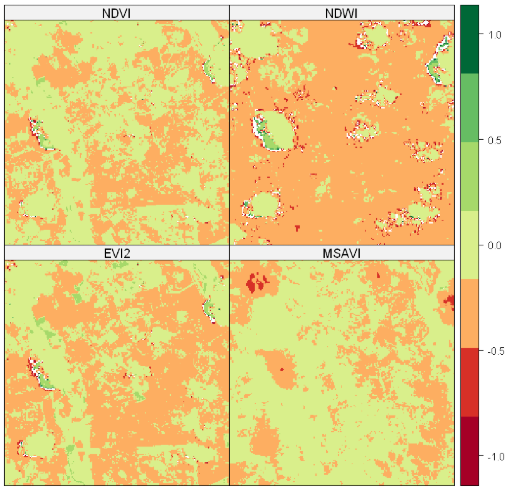
\includegraphics[width=0.97\linewidth]{FIGURAS/indices20131023}
 					\label{fig:ima2013} 
 				\end{figure}			
 				
 			\end{minipage}\hfill
 			\begin{minipage}[t!]{0.31\textwidth}
 				
 				\begin{figure}[H]
 					\centering \small \caption{2016}
 					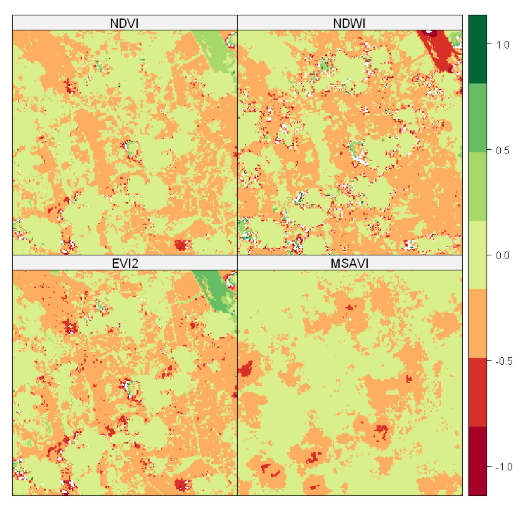
\includegraphics[width=0.97\linewidth]{FIGURAS/indices20160101}
 					\label{fig:inda15} 
 				\end{figure}			
 				
 			\end{minipage} 
 			\begin{minipage}[t!]{0.31\textwidth}
 				
 				\begin{figure}[H]
 					\centering \small \caption{2023}
 					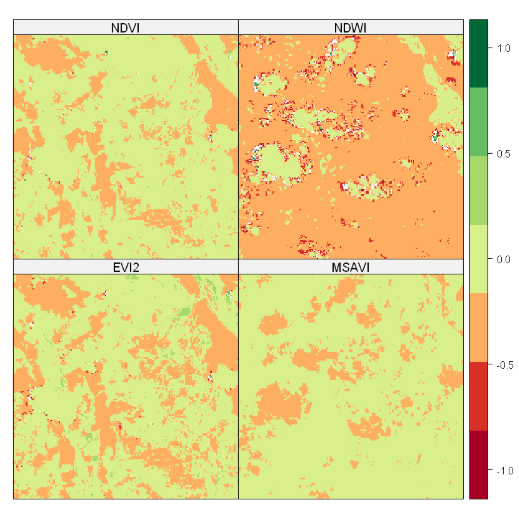
\includegraphics[width=0.97\linewidth]{FIGURAS/indices20231222}
 					\label{fig:inda2023} 
 				\end{figure}		
 			\end{minipage} 
 			
 			\begin{center}
 				Fonte:   Elaborado pelos Autores (2025)
 			\end{center}
 			% }}}
 \hspace*{1.25 cm} Neste conjunto de imagens em nível de cinza,  escolhido a paleta de cores "RdYlGn" do "package ViridisLite" nas Figuras \ref{fig:rplot-ndwi2016} a \ref{fig:difer202332026}, cujas as  medidas pelo sensor e transformadas aos índices espectrais, demonstram que a água ocorreu maior variação neste índice medido e calculado, e por nisso o índice NDWI  foi escolhido para uma análise mais priorizada.   \\
  % {{{   
 			\begin{minipage}[t!]{0.31\textwidth}
 				\begin{figure}[H]
 					\centering \small \caption{NDWI 2016}
 					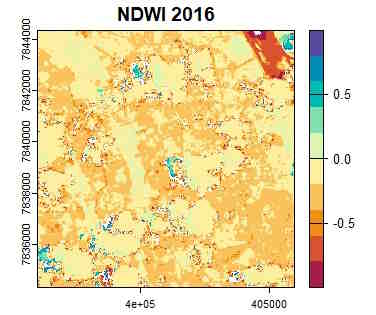
\includegraphics[width=0.97\linewidth]{FIGURAS/Rplotndwi2016}
 					\label{fig:rplot-ndwi2016}
 				\end{figure}			
 				
 			\end{minipage}\hfill
 			\begin{minipage}[t!]{0.31\textwidth}
 				
 				\begin{figure}[H]
 					\centering \small \caption{NDWI 2023}
 					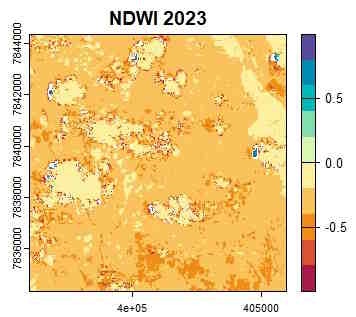
\includegraphics[width=0.97\linewidth]{FIGURAS/Rplot0ndwi2023}
 					\label{fig:rplot0ndwi2023}
 				\end{figure}			
 				
 			\end{minipage} 
 			\begin{minipage}[t!]{0.31\textwidth}
 				
 				\begin{figure}[H]
 					\centering \small \caption{Diferenças no NDWI}
 					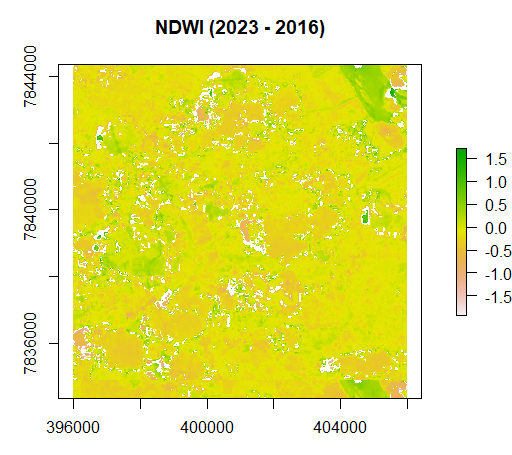
\includegraphics[width=0.97\linewidth]{FIGURAS/difer202332026}
 					\label{fig:difer202332026}
 				\end{figure}		
 			\end{minipage} 
 			
 			\begin{center}
 				Fonte:   Elaborado pelos Autores (2025)
 			\end{center}
 			% }}}		
	%	
 \hspace*{1.25 cm}  Ao destacarmos o índice NDWI nas duas imagens com diferença temporal de 8(oito)anos, temos a Figura   \ref{fig:difer202332026} e nesta a atenção pode ser observada no canto superior direito, e em outras superfícies com maior presença de água, como brejos e açudes, a alteração contrastante destas diferenças.  \\
 %------------------
  \begin{wrapfigure}{r}{0.65\textwidth}
	\begin{center}
		\centering  \small \caption{Amostragem em grid}
		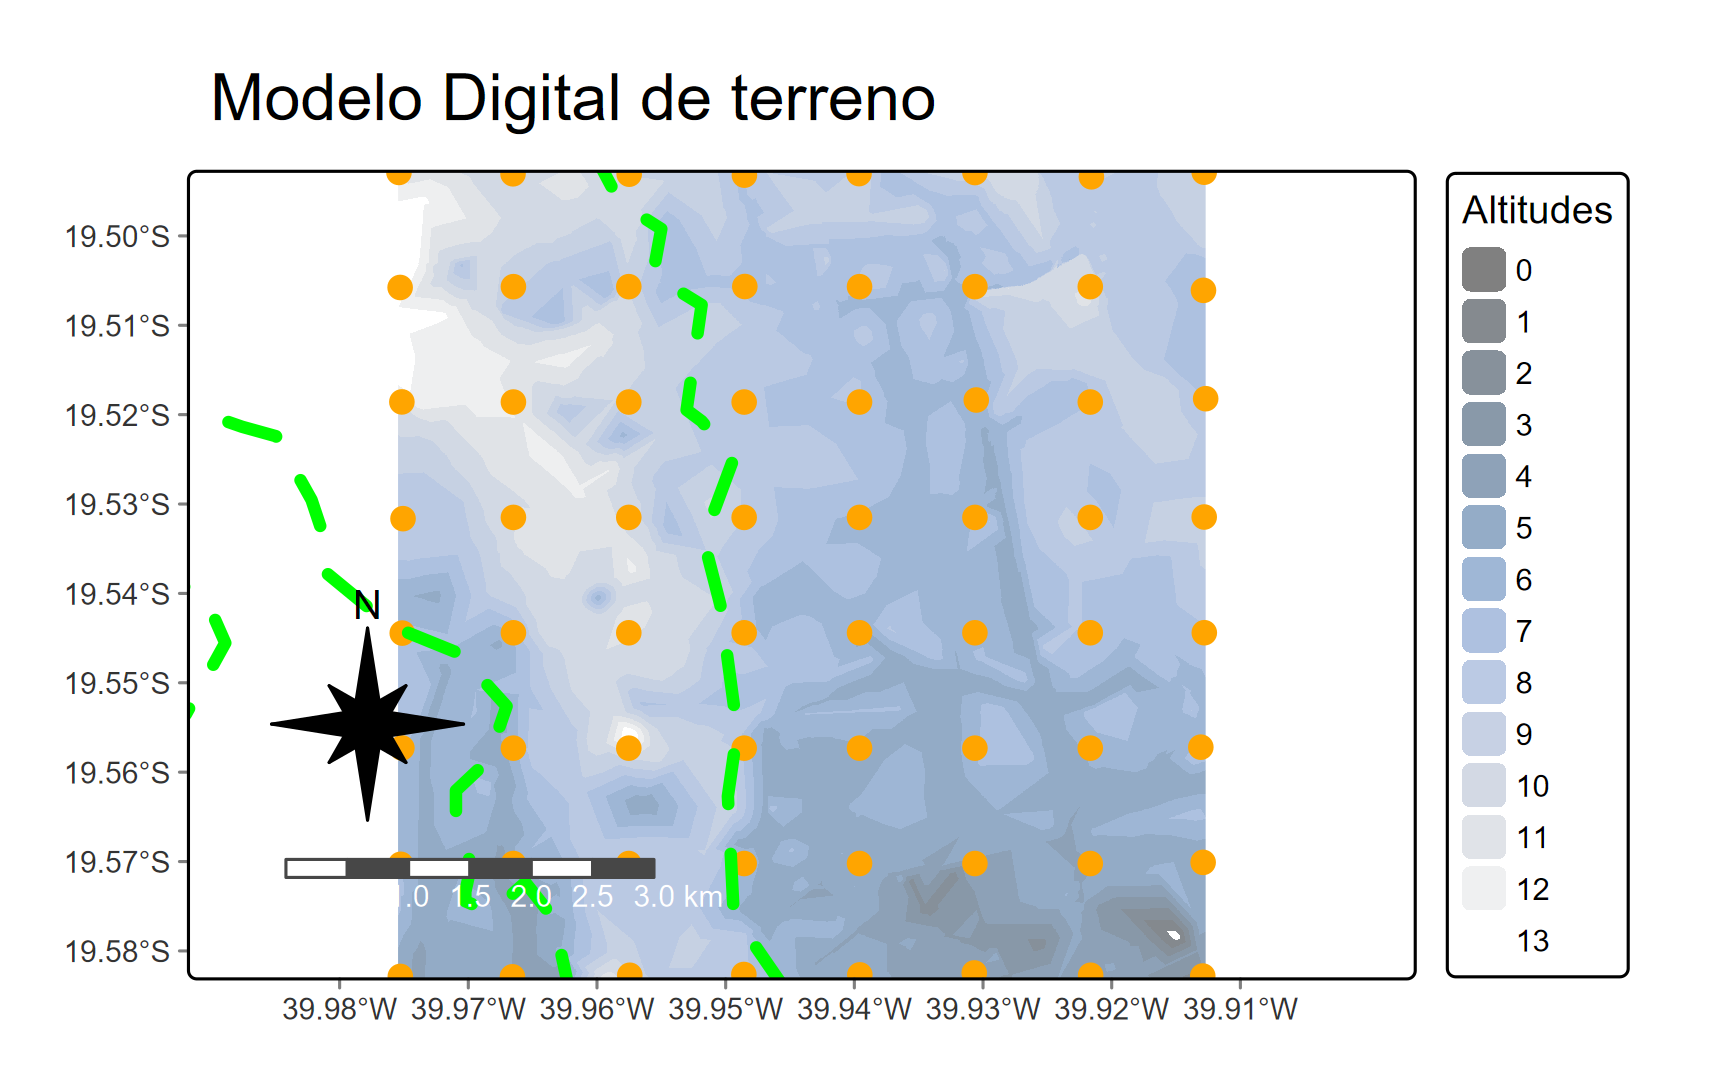
\includegraphics[width=0.97\linewidth]{FIGURAS/mdtamostras}
		\label{fig:mdtamostras}\\{ Fonte:   Elaborado pelos Autores (2025)}
	\end{center}
\end{wrapfigure} 

 %------------------
  \hspace*{1.25 cm}  Neste momento, a percepção do objeto observado ser uma superfície, quase continua(excluídos vazios radiométricos), torna-se inerente ao fenômeno de estudo. E por ser uma superfície, com valores máximos, mínimos, direção, desvio padrão e variância do valor do índice com coordenada (x,y). Deve ser tratada como tal, e ser analisadas  por técnicas da geoestátistica.   \\
  %------------------
  \hspace*{1.25 cm}  Ao decimo sétimo e oitavo paragrafo da seção 3, ao descrevermos a estrutura de amostragem, e ao parágrafo anterior  que  compreendemos a estrutura do fenômeno com uma \underline{variável regionalizada}, e por isso voltamos a  \cite[p.10]{Yamamoto} :
\begin{quoting}[rightmargin=0cm,leftmargin=4cm]
	\begin{singlespace}
		{
			\textit{Os métodos geoestatísticos fornecem um conjunto de técnicas necessárias para entender a aparente aleatoriedade dos dados, os quais apresentam, porém, uma possível estruturação espacial, estabelecendo, desse modo, uma função de correlação espacial.}
		}
	\end{singlespace}
\end{quoting} 
 %------------------
 \hspace*{1.25 cm} Ainda em  \cite[p.19 e 20]{Yamamoto}, o fenômeno estudado se comporta dentro de domínios, sejam em 2D ou 3D, e apresentam distribuição e variabilidade espaciais. A "metodologia da geoestátistica se destaca ao oferecer a incerteza associada à estimativa" \\
 %
  \hspace*{1.25 cm} Continuando em  \cite[p.20 e 21]{Yamamoto}, na "\textit{reprodução das característica do fenômeno espacial baseado em pontos amostrais é denominado interpolação ou estimativa}". O processo de para inferir a distribuição e a variabilidade espacial, vai  depender do tamanho da amostra e da distribuição espacial, e em nosso caso se estabeleceu tanto por aleatoriedade Figura \ref{fig:usoSOLOamostras} e Figura \ref{fig:mdtamostras} \\
 %
  \hspace*{1.25 cm}  Coletado os dados, e tabulados, necessitamos fazer a sumarização e analise exploratória,  no entanto varias vezes verificamos  situações que impossibilita termos conclusões sobre os seus resultados. E como em  \cite[p.18]{Webster}, muitas variáveis ambientais, principalmente nas  concentradas no solo, estão na forma de distribuição normal, de acordo com as "\textit{descoberta independentemente por De Moivre, Laplace e Gauss, mas Gauss parece geralmente levar o crédito por ela. E a distribuição é frequentemente chamada de "gaussiana"}". \\
%
  \hspace*{1.25 cm}  Ainda em \cite[p.20]{Webster}, mas a utilização destes dados na formulação de modelos, apresentam dificuldades, podemos transformar os valores medidos a uma nova escala, "\textit{se necessário, transformar os resultados para a escala original ao final}." \\
 % 
\hspace*{1.25 cm}  Na Figura \ref{fig:difer202332026} realizando operações de interpolação com a utilização do grid, conseguimos obter uma imagem com alguma normalidade, Figura \ref{fig:RplotN16}. No entanto ao aplicarmos o \textbf{\textcolor{blue}{bestnormalize}}, os resultado é surpreendente, tanto que apresentamos em Figura \ref{fig:RplotMELNHOR}, e nos estimulou a geração do modelo matemático em 3D, Figura \ref{fig:RplotP34}\\
%---------------- 
  % {{{   
 			\begin{minipage}[t!]{0.31\textwidth}
 				\begin{figure}[H]
 					\centering \small \caption{Antes da normalização}
 					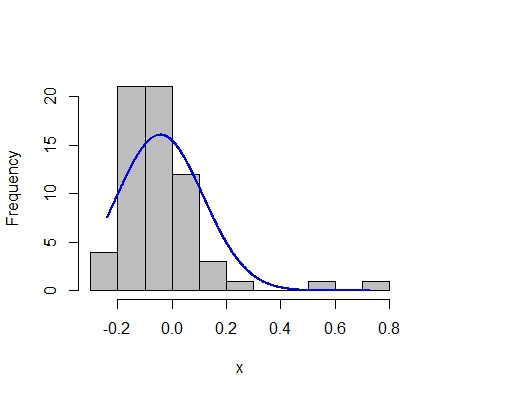
\includegraphics[width=0.97\linewidth]{FIGURAS/RplotN1}
 					\label{fig:RplotN16}
 				\end{figure}			
 				
 			\end{minipage}\hfill
 			\begin{minipage}[t!]{0.31\textwidth}
 				
 				\begin{figure}[H]
 					\centering \small \caption{Apôs a normalização}
 					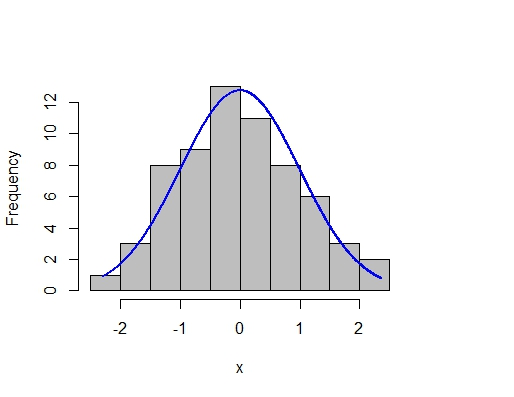
\includegraphics[width=0.97\linewidth]{FIGURAS/RplotMELNHOR}
 					\label{fig:RplotMELNHOR}
 				\end{figure}			
 				
 			\end{minipage} 
 			\begin{minipage}[t!]{0.31\textwidth}
 				
 				\begin{figure}[H]
 					\centering \small \caption{Perspectiva da Superfície}
 					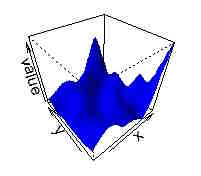
\includegraphics[width=0.97\linewidth]{FIGURAS/RplotP34}
 					\label{fig:RplotP34}
 				\end{figure}		
 			\end{minipage} 
 			
 			\begin{center}
 				Fonte:   Elaborado pelos Autores (2025)
 			\end{center}
 			% }}}
 %%--------------
 \lstset{
	language=R, % Define a linguagem como JavaScript
	caption= Sujestões de melhoria ao modelo em  linguagem R} % Legenda do código
\begin{lstlisting}[language=R]
 Best Normalizing transformation with 64 Observations
Estimated Normality Statistics (Pearson P / df, lower => more normal):
- arcsinh(x): 1.7857
- Center+scale: 1.8024
- Double Reversed Log_b(x+a): 1.7667
- Exp(x): 1.9929
- Log_b(x+a): 1.5042
- orderNorm (ORQ): 1.4643
- sqrt(x + a): 1.2955
- Yeo-Johnson: 1.2452
Estimation method: Out-of-sample via CV with 10 folds and 5 repeats 
Based off these, bestNormalize chose:
Standardized Yeo-Johnson Transformation with 64 nonmissing obs.:
Estimated statistics:
- lambda = -3.643204 
- mean (before standardization) = -0.09376124 
- sd (before standardization) = 0.1402468
\end{lstlisting}  
% 
\hspace*{1.25 cm} A produção inicial do variograma,  com procedimentos em \cite[p.224]{Bivand}, com a caracterização mensurada e sua distância em visão inicial da análise em Figura \ref{fig:variinical}\\
 %%%===================
 \begin{minipage}[t!]{0.5\textwidth}
 	\begin{figure}[H]
 		\centering \small \caption{Semivariograma sem definição do modelo explicativo}
 		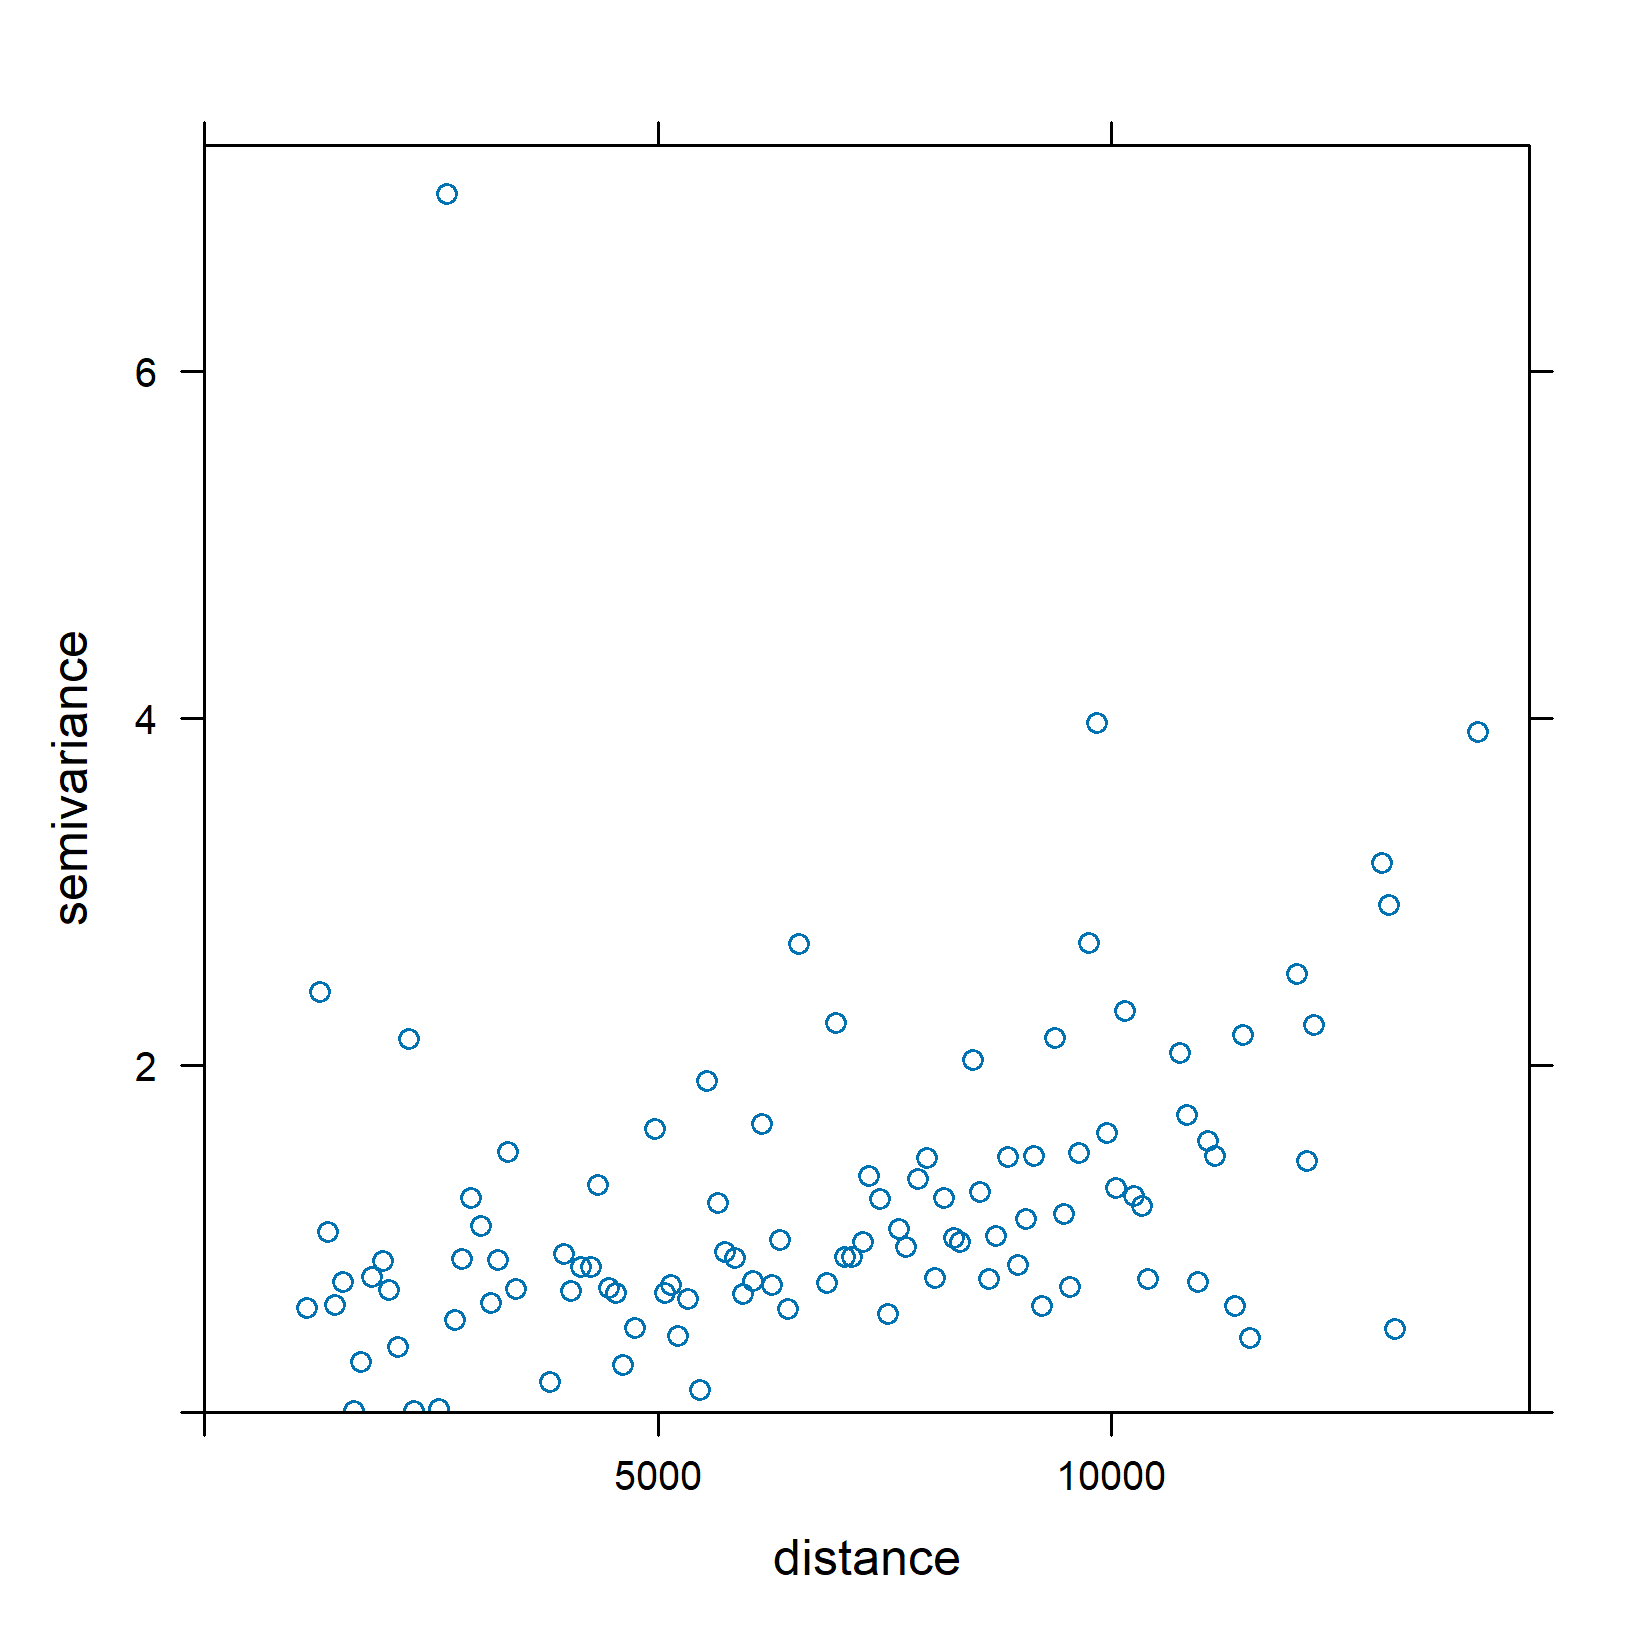
\includegraphics[width=0.97\linewidth]{FIGURAS/variogramaPTONOS}
 		\label{fig:variinical}
 	\end{figure}	
 \end{minipage}\hfill
 \begin{minipage}[t!]{0.5\textwidth}
 	\begin{figure}[H]
 		\centering \small \caption{Modularização da reflectância}
 		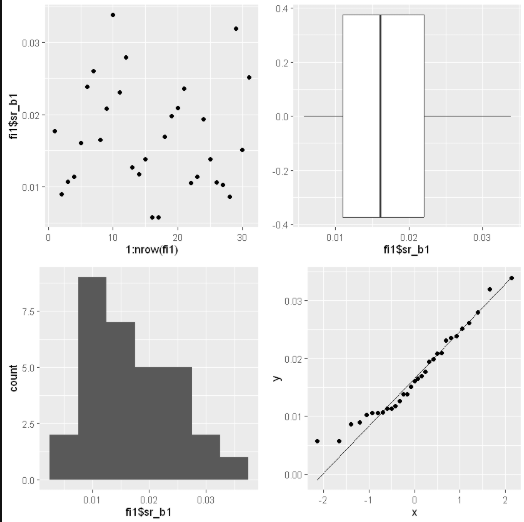
\includegraphics[width=0.97\linewidth]{FIGURAS/normali}
 		\label{fig:Rplothdg}
 	\end{figure}		
 \end{minipage} 
 % {{{   			
 			\begin{center}
 				Fonte:   Elaborado pelos Autores (2025)
 			\end{center}
 			% }}
 %==========================================		
%\hspace*{1.25 cm} E seu modelo de superfície plana, pode ser apreciado em Figura \ref{fig:superficie} critérios que podem também ser observados em Figura \ref{fig:superficie1} e sua melhora e Figura  \ref{fig:Rplothdg}\\
 		 %%-------------- 
  \hspace*{1.25 cm} A escolha da função matemática que produza, e nos possibilite a explicar o modelo, pode ser encontrada em  \cite[p.90]{delgado}, e a mesma deve ser inserido os parâmetros e efeitos, com o significado em língua inglesa que são o patamar ("sill"), pepita("nugget"), comprimento("range") e sua contribuição("contribution") .	\\	
 		 %%-------------- 
% {{{   
			\begin{minipage}[t!]{0.31\textwidth}
				\begin{figure}[H]
					\centering \small \caption{ Escolha da função }
					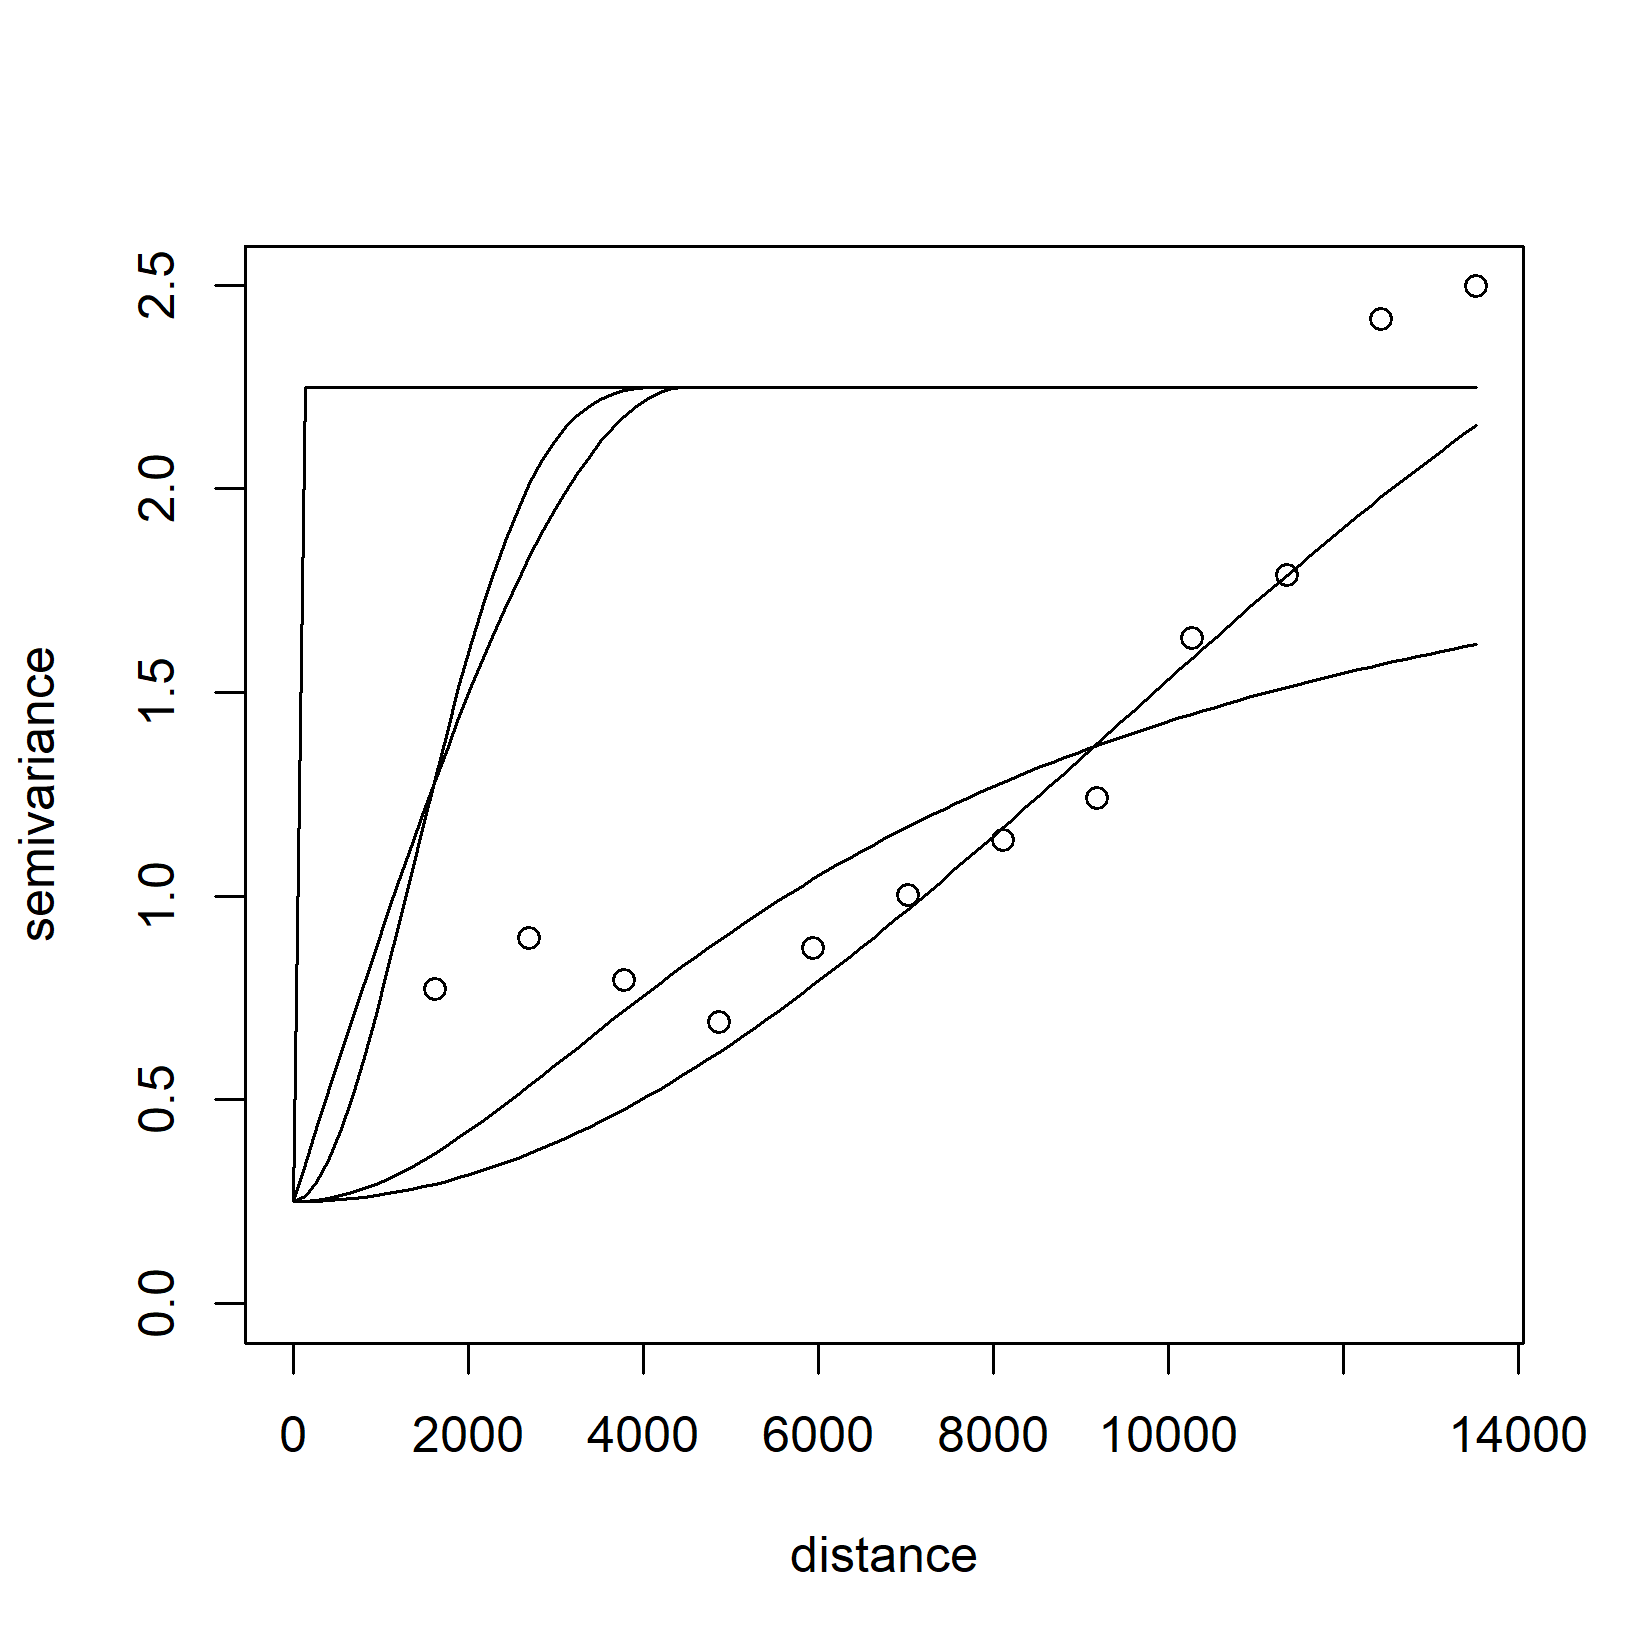
\includegraphics[width=0.97\linewidth]{FIGURAS/variogramageor4}
					\label{fig:variogramageor4}
				\end{figure}			
				
			\end{minipage}\hfill
			\begin{minipage}[t!]{0.31\textwidth}
				
				\begin{figure}[H]
					\centering \small \caption{Modelo esférico}
					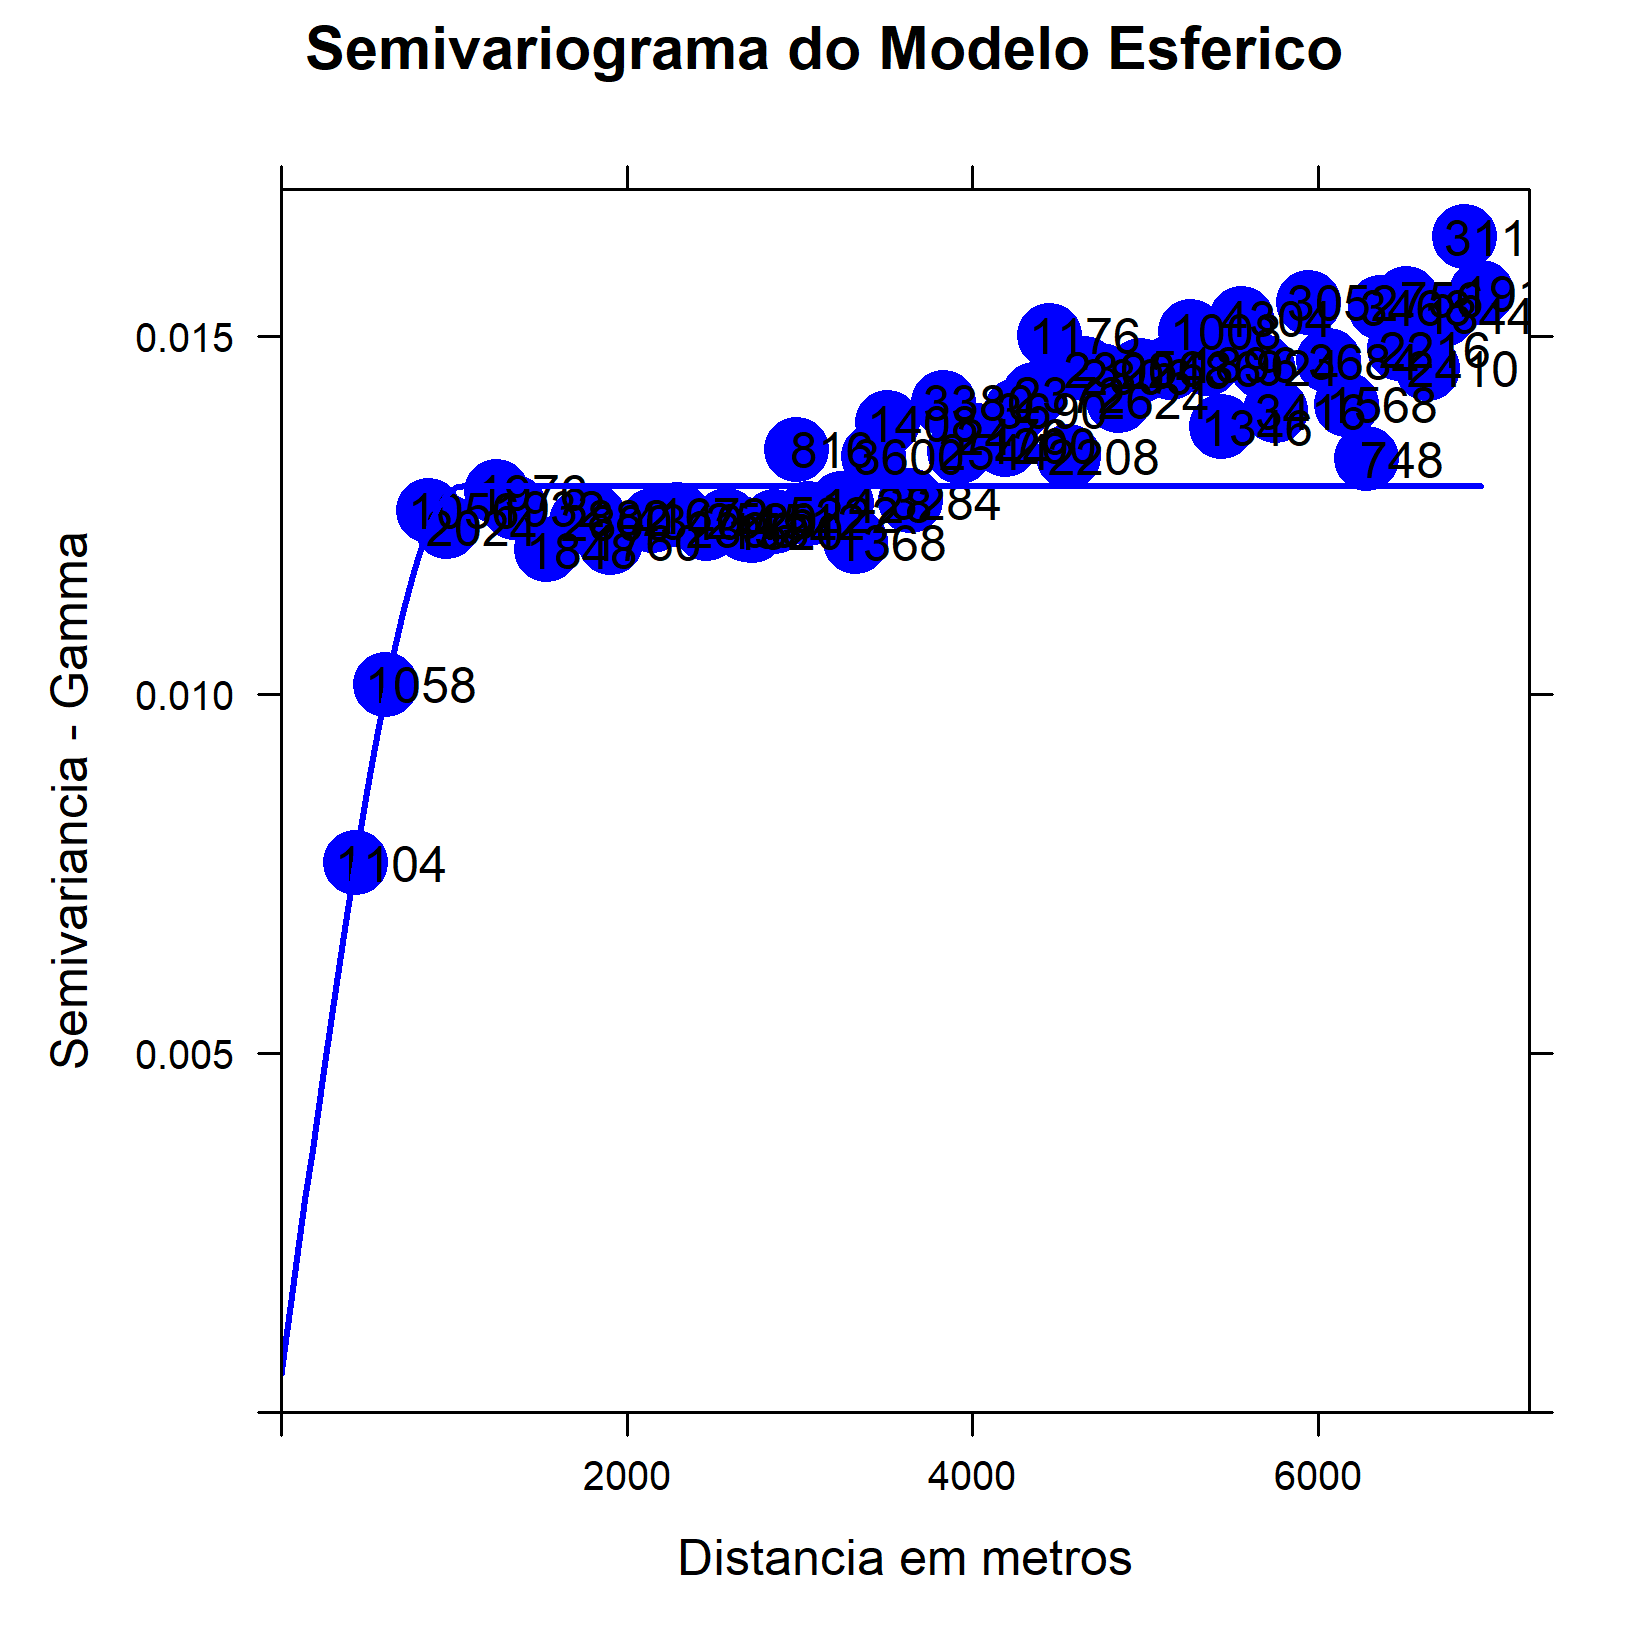
\includegraphics[width=0.97\linewidth]{FIGURAS/modelos-esferico}
					\label{fig:varexpfitsp}
				\end{figure}			
				
			\end{minipage} 
			\begin{minipage}[t!]{0.31\textwidth}
				
				\begin{figure}[H]
					\centering \small \caption{Validação cruzada}
					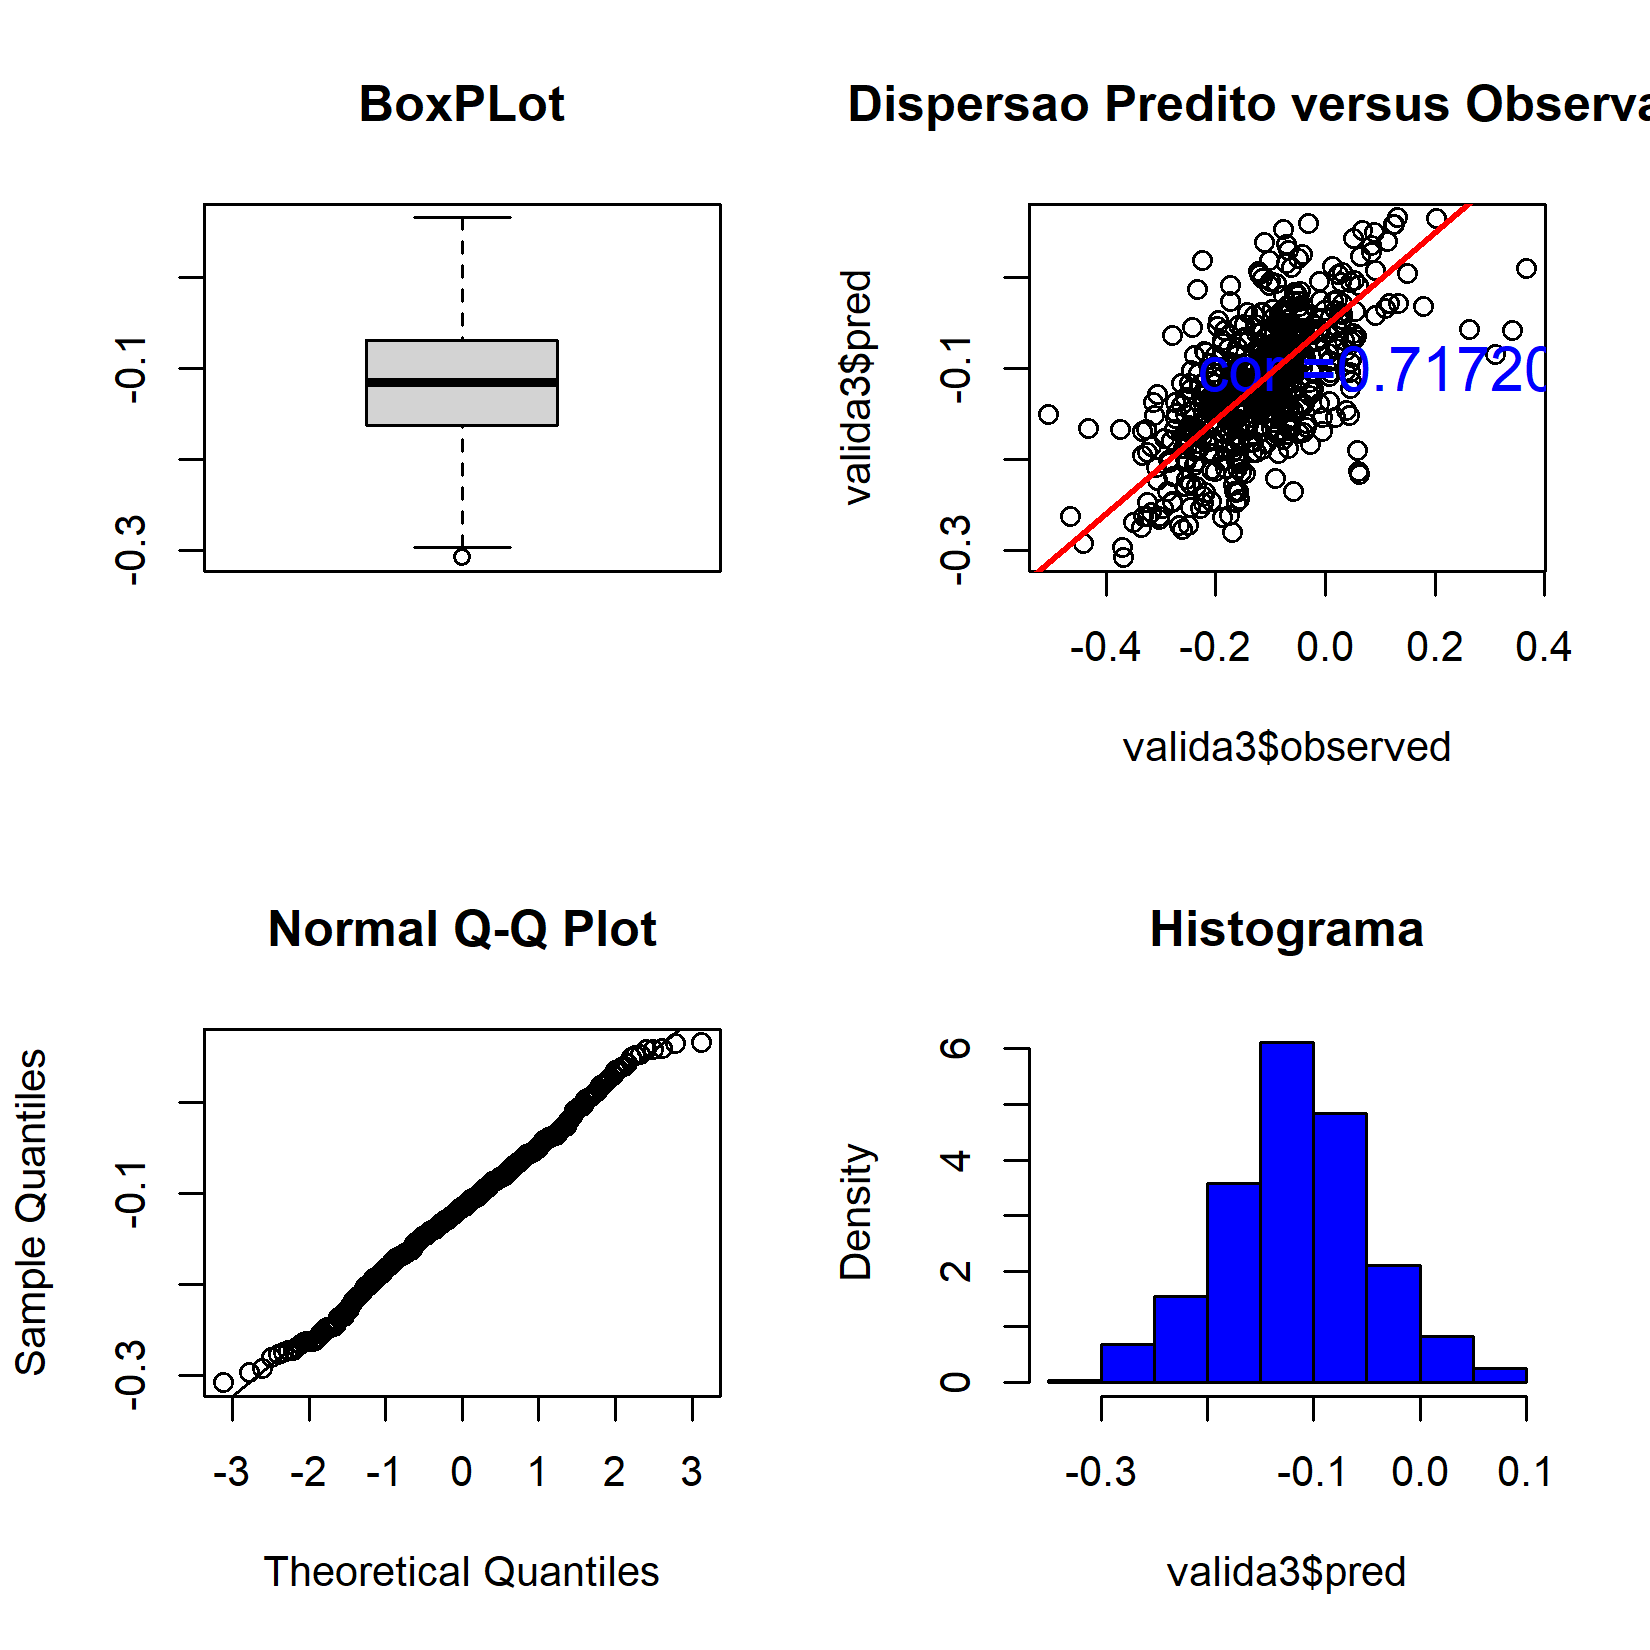
\includegraphics[width=0.97\linewidth]{FIGURAS/valicas}
					\label{fig:xvalid.cruzadaesferica2}
				\end{figure}		
			\end{minipage} 
			
			\begin{center}
				Fonte:   Elaborado pelos Autores (2025)
			\end{center}
			% }}
 \hspace*{1.25 cm} 	Em todas as Figuras \ref{fig:variinical} e \ref{fig:superfdicie} que a estacionáriedade  inicia-se visualmente em aproximadamente em 0,9 e seu "range" em torno de 1300 metros\\
 %		
 \hspace*{1.25 cm} Na Figura \ref{fig:variogramageor4} o processo da escolha da função, na Figura \ref{fig:varexpfitsp} a função escolhida, e finalmente na Figura \ref{fig:xvalid.cruzadaesferica2} a validação cruzada, com a regressão em homocedasticidade\\
 %%-------------- 
 \hspace*{1.25 cm} Em Figura \ref{fig:superfdicie}, temos a superfície da interpolação, com a analise da covariância do modelo, distribuído espacialmente em Figura \ref{fig:htrrtyR} , com procedimentos vistos em   \cite[p.47]{delgado}, e como cada variável, seus resíduos, e observação contribuem na explicação do modelo em \ref{fig:Rplothddg} \\
   % {{{   
 			\begin{minipage}[t!]{0.31\textwidth}
 				\begin{figure}[H]
 					\centering \small \caption{Superfície interpolada}
 					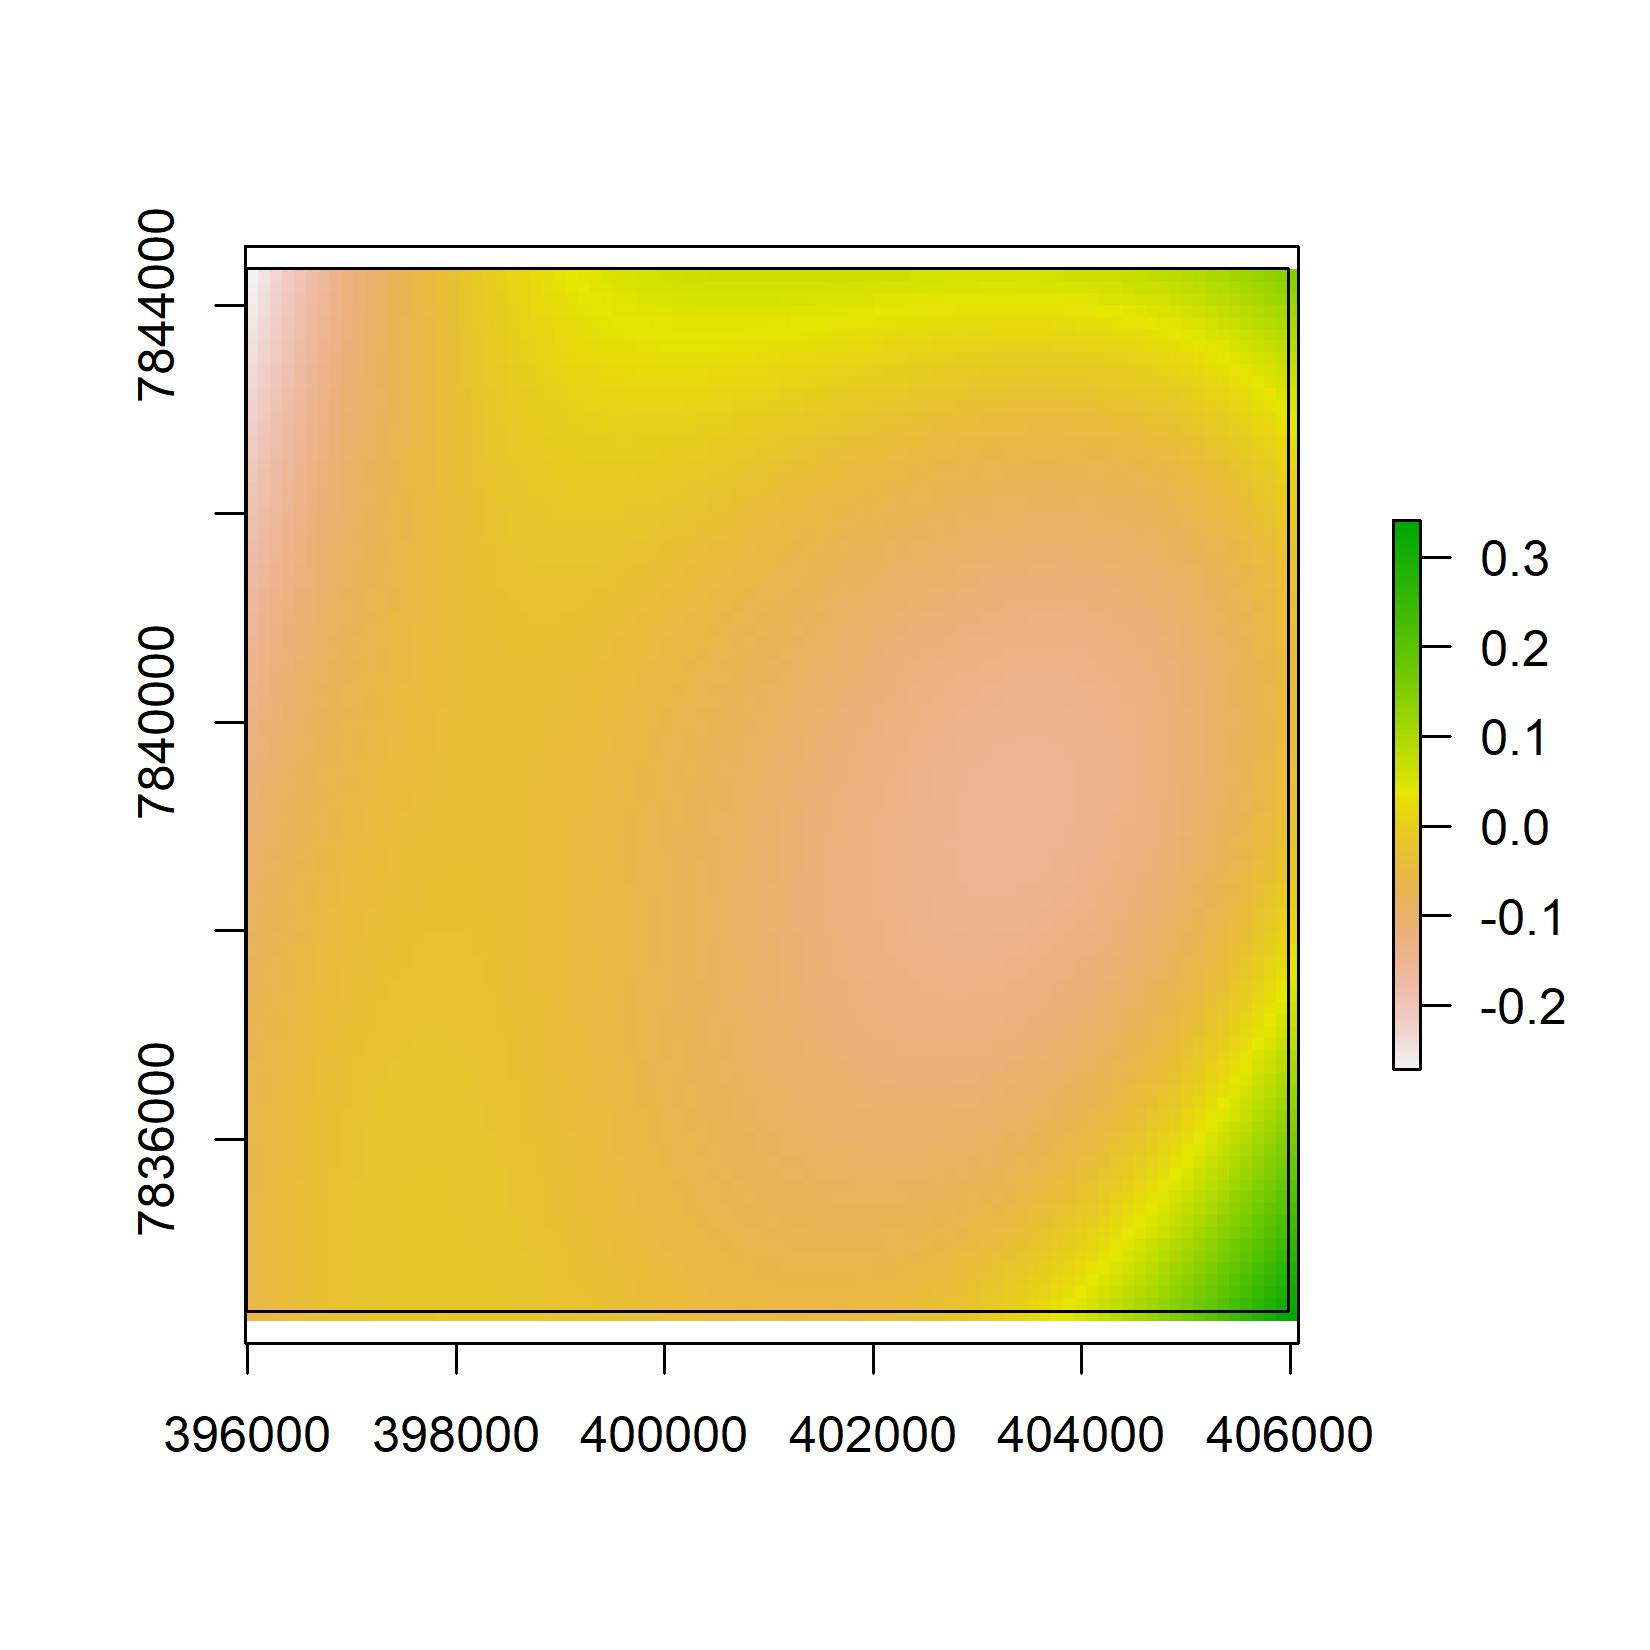
\includegraphics[width=0.97\linewidth]{FIGURAS/superficie}
 					\label{fig:superfdicie}
 				\end{figure}			
 				
 			\end{minipage}\hfill
 			\begin{minipage}[t!]{0.31\textwidth}
 				
 				\begin{figure}[H]
 					\centering \small \caption{Modelo esférico}
 					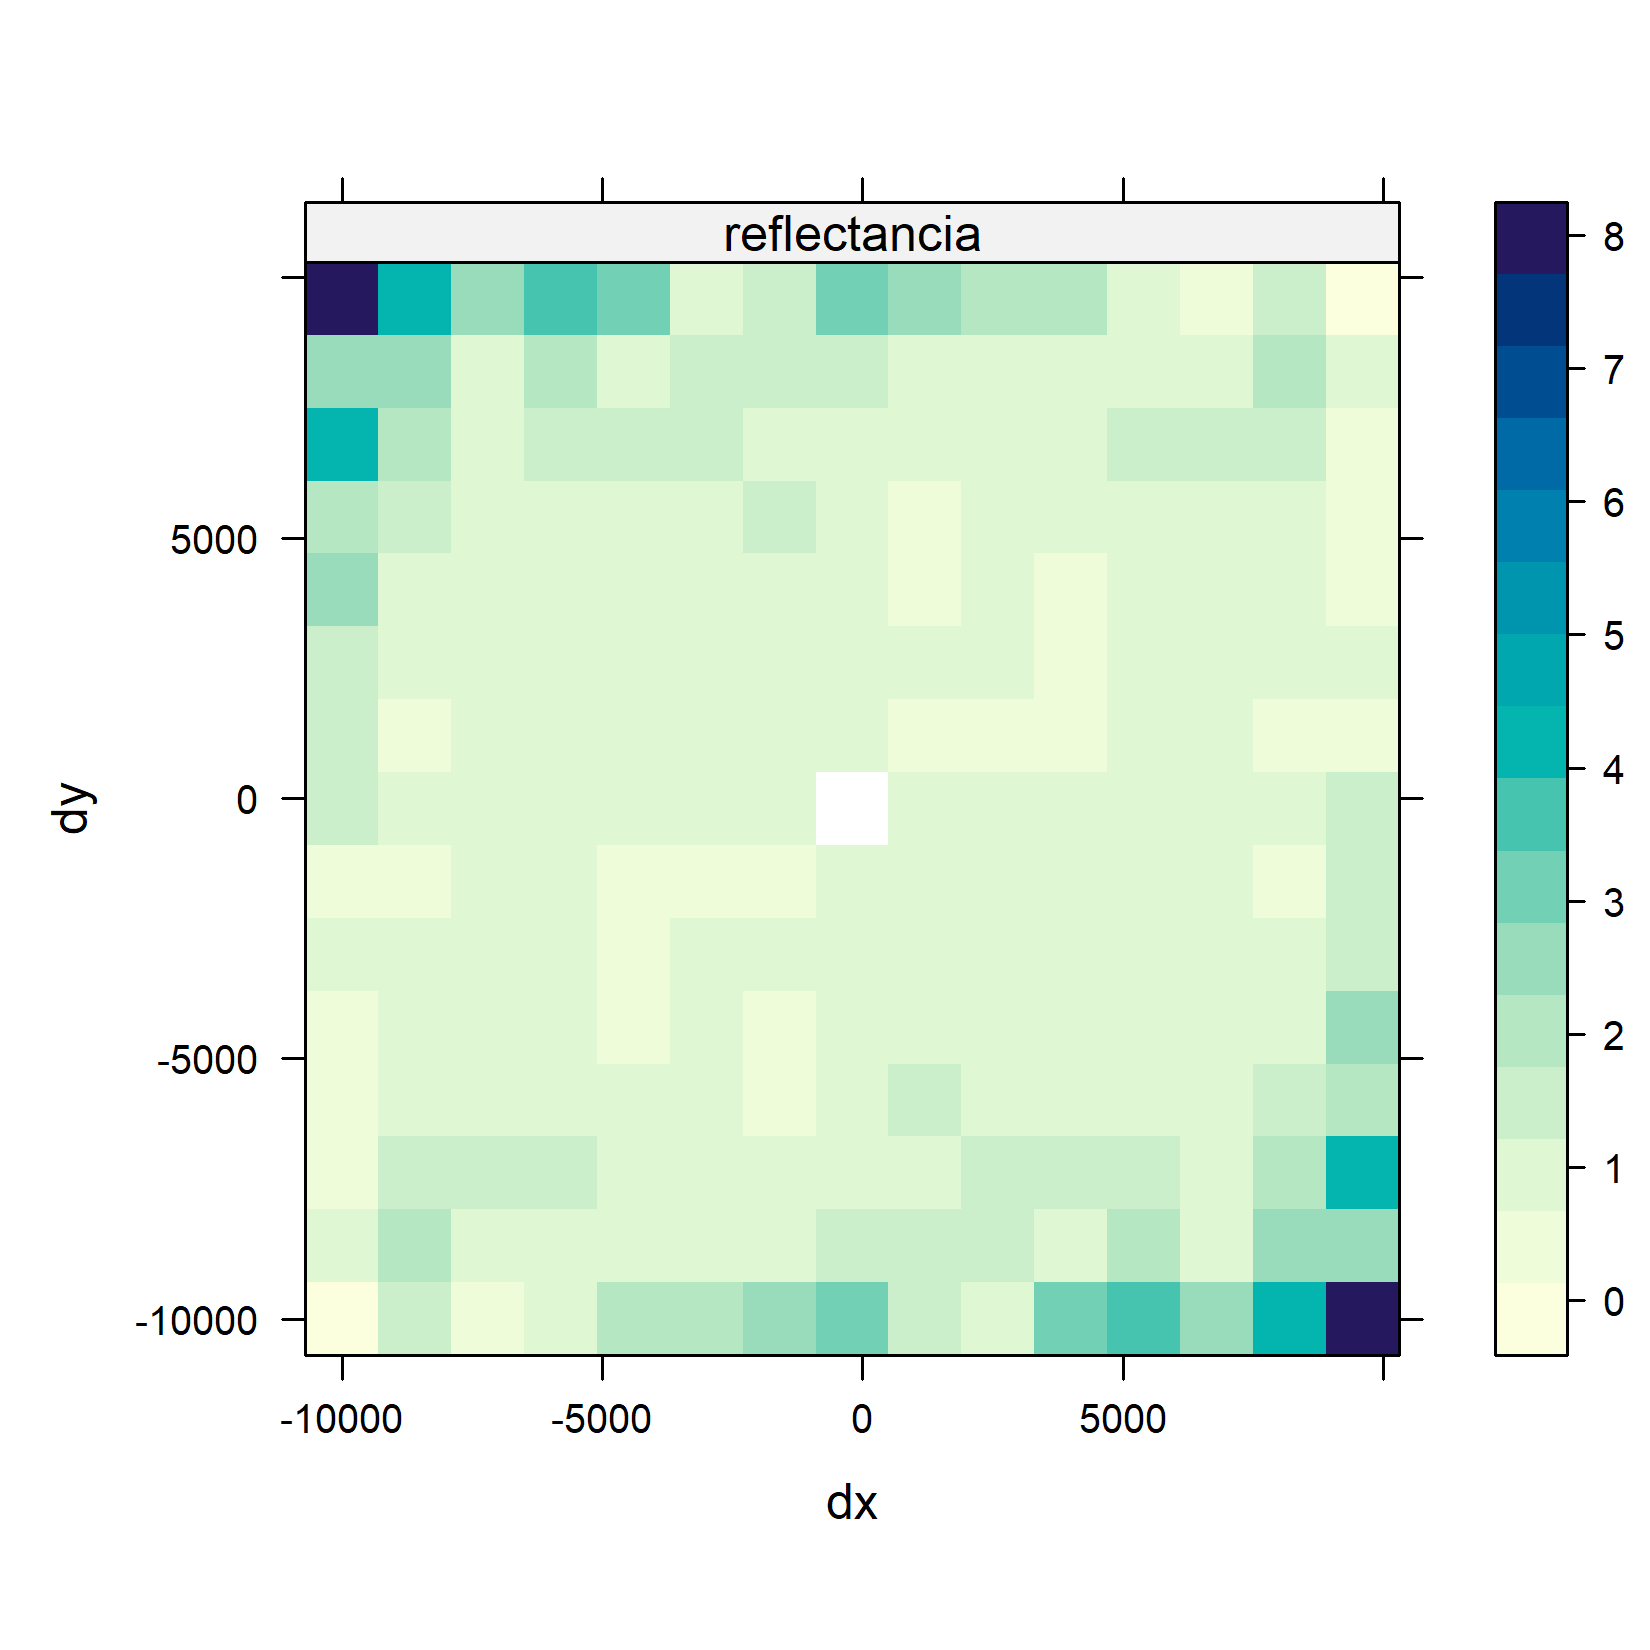
\includegraphics[width=0.97\linewidth]{FIGURAS/varexpmap}
 					\label{fig:htrrtyR}
 				\end{figure}			
 				
 			\end{minipage} 
 			\begin{minipage}[t!]{0.31\textwidth}
 				
 				\begin{figure}[H]
 					\centering \small \caption{Contribuição espacial das variável mensurada}
 					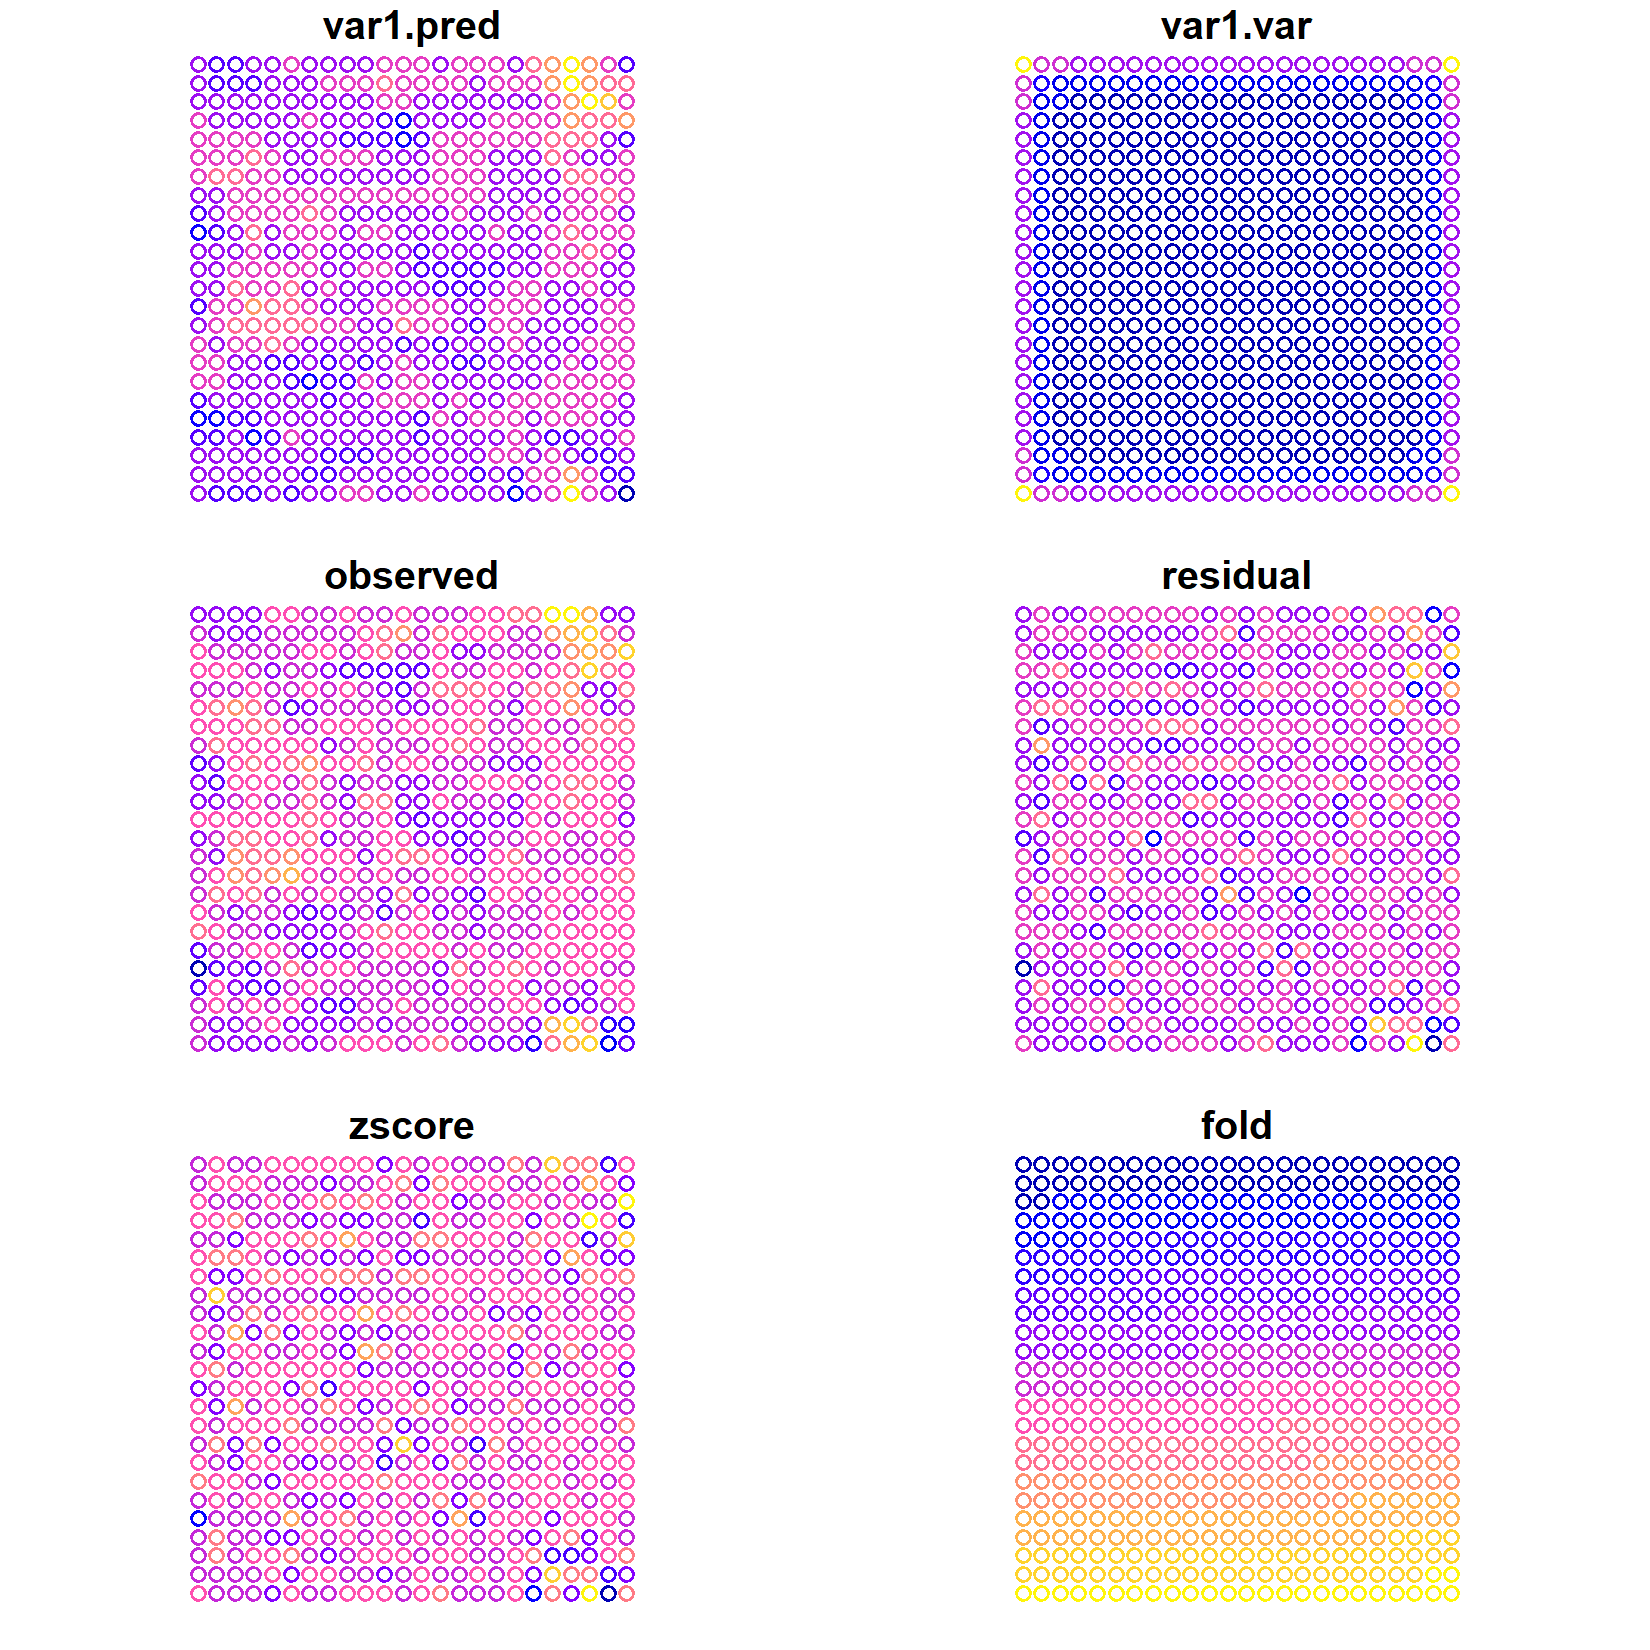
\includegraphics[width=0.97\linewidth]{FIGURAS/xvalid.sph-map}
 					\label{fig:Rplothddg}
 				\end{figure}		
 			\end{minipage} 
 			
 			\begin{center}
 				Fonte:   Elaborado pelos Autores (2025)
 			\end{center}
 			% }}

\hspace*{1.25 cm} Dando o enfoque no modelo esférico,  determinados enfase nos parâmetros deste modelo. E passo que escolhemos o modelo, sendo que o resultado erro médio quadrático  e a porcentagem explicada do modelo em quadra a seguir. 
%%
\lstset{
	language=R, % Define a linguagem como R
	caption= Resultado do modelo de superficie de tendencia de 3 grau saida da linguagem R} % Legenda do código
\begin{lstlisting}[language=R]
.0364868216565002  # root mean squared error
A matrix: 1 × 1 of type dbl
0.9465385  # % de explicacao do modelo
\end{lstlisting}   
  \begin{wrapfigure}{l}{0.506\textwidth}
	\begin{center}
		\centering  \small \caption{Modelagem por krigagem}
		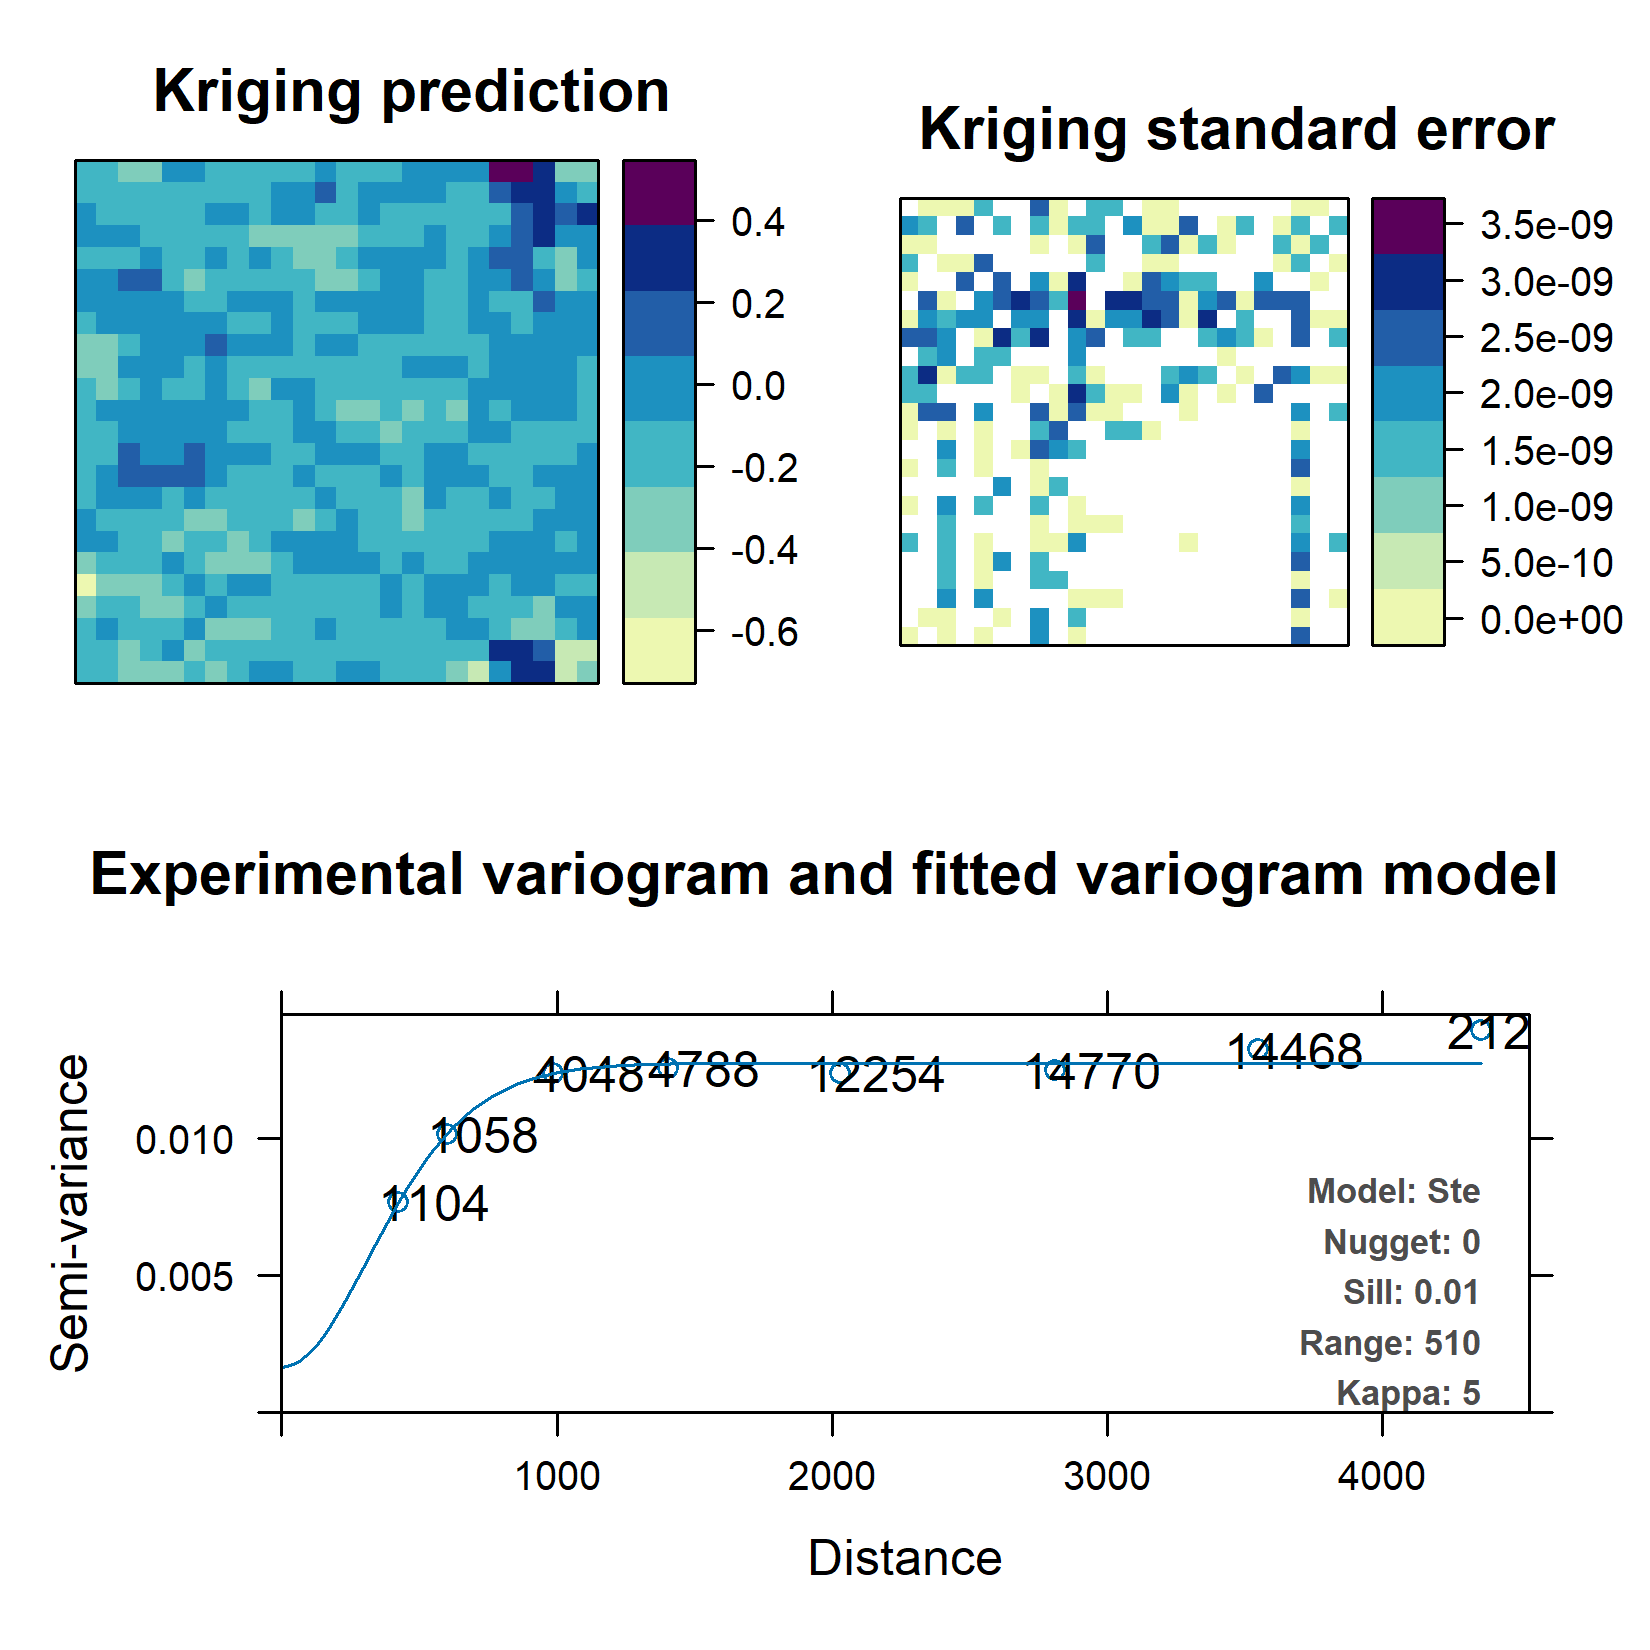
\includegraphics[width=0.97\linewidth]{FIGURAS/MODELOKRIGAGEM-MELHOR}
		\label{fig:rplotkriga}\\{ Fonte:   Elaborado pelos Autores (2025)}
	\end{center}
\end{wrapfigure} 	 


 \begin{comment}
 	\begin{figure}[H]
 		\centering  \small \caption{Modelagem por krigagem}
 		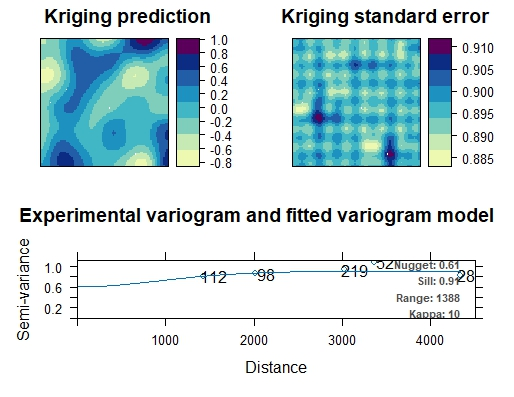
\includegraphics[width=0.57\linewidth]{FIGURAS/Rplotkriga}
 		\label{fig:rplotkriga}\\{ Fonte:   Elaborado pelos Autores (2025)}
 	\end{figure}
 	
 	%%%%%%%%%%%%%%%%%%%%%%%%%%%%%%%%%%%

 \end{comment}
  
\hspace*{1.25 cm} O que nos animou a elaboração da krigagem em Figura \ref{fig:rplotkriga}, o que possibilita ao lado direito da figura os locais onde ocorrem os maiores erros, na determinação desta superfície. E para também o variograma ficou próximo ao da Figura \ref{fig:Rplothddg}  \\
 
 \begin{comment}
\begin{figure}
	\centering
	\caption{}
	\label{fig:rplotndwi2016}
	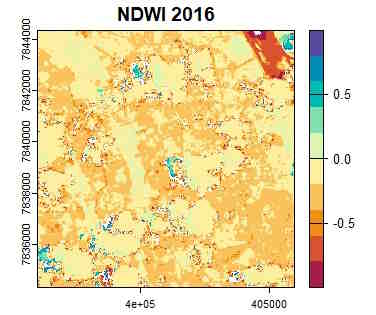
\includegraphics[width=0.97\linewidth]{FIGURAS/Rplotndwi2016}
\end{figure}
 	\begin{center}
 		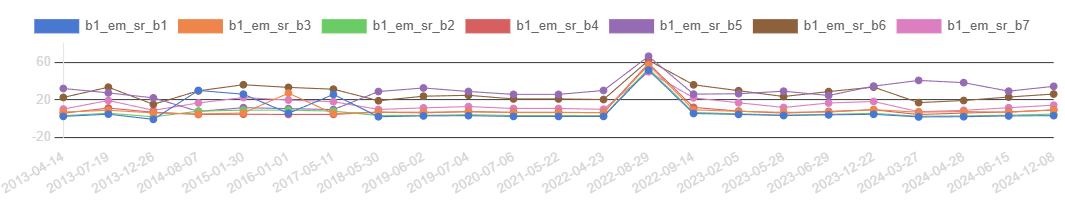
\includegraphics[width=0.97\linewidth]{FIGURAS/pontoB1}
 	\end{center}
 	\begin{center}
 		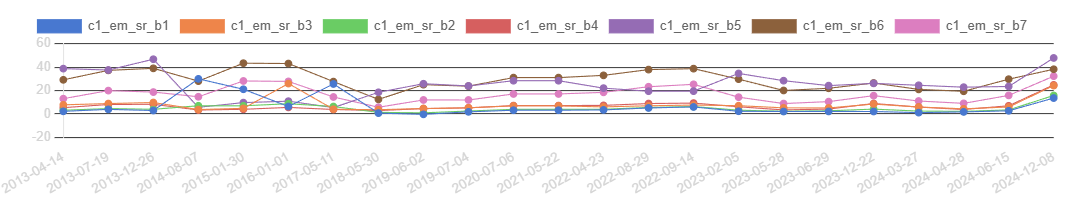
\includegraphics[width=0.97\linewidth]{FIGURAS/pontoC1}
 	\end{center}
 	\begin{center}
 		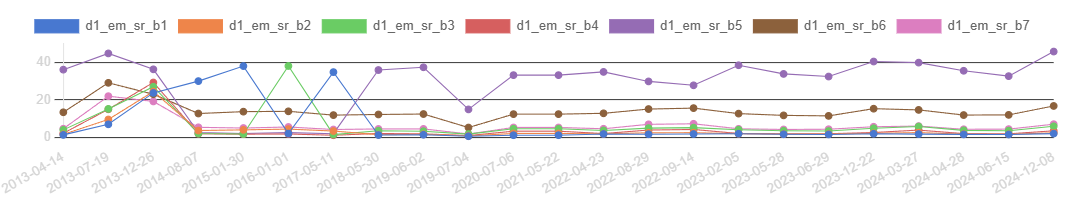
\includegraphics[width=0.97\linewidth]{FIGURAS/PontoD1}
 	\end{center}
 	
 \end{comment}
\hspace*{1.25 cm} E finalmente, passamos para a análise temporal, o qual escolhemos uma posição geográfica onde ocorrem uma maio variação deste modelo superficial de variações de reflectância, pode análise temporal entre as diferenças  \( \Delta T = T_{2}  - T_{1} \)\\
%
\hspace*{1.25 cm}  Na Figura \ref{fig:INDICES}, mostra o comportamento anômalo de todos os índices espectrais ao inicio do ano de 2016, junto a margem.\\

 \begin{figure}[H]
	\centering  \small \caption{Índices em  análise temporal}
	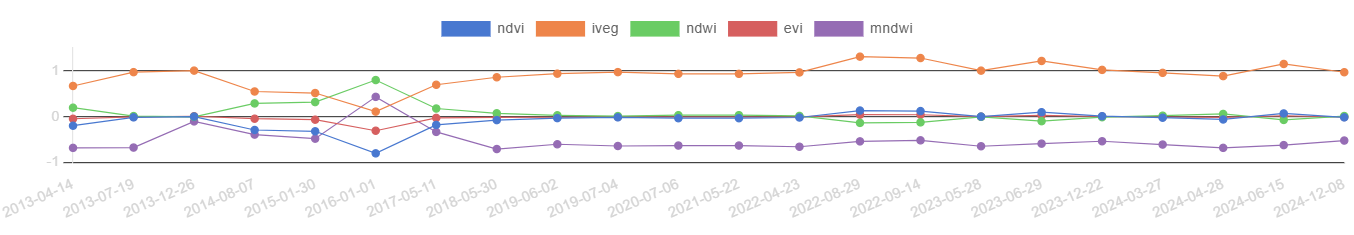
\includegraphics[width=0.97\linewidth]{FIGURAS/indices}
	\label{fig:INDICES}{ Fonte:   Elaborado pelos Autores (2025)}
\end{figure}

 \begin{figure}[H]
	\centering  \small \caption{Aumento do óxido de ferro no período}
	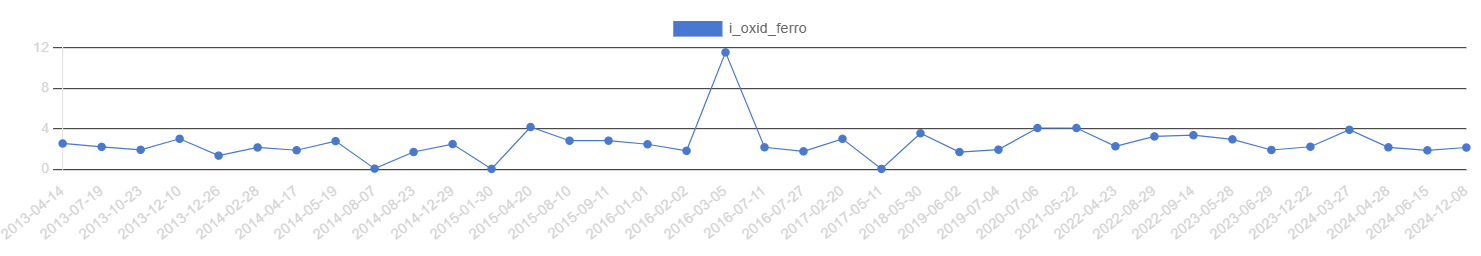
\includegraphics[width=0.97\linewidth]{FIGURAS/graphvisualiser-1747928533564}
	\label{fig:INDICES2}{ Fonte:   Elaborado pelos Autores (2025)}
\end{figure}

\hspace*{1.25 cm} A variação do óxido de ferro alcançou o máximo ao ano de 2018 como Figura \ref{fig:INDICES2}\\
%
\begin{figure}[H]
	\centering  \small \caption{Índices NDVI e NDWI}
	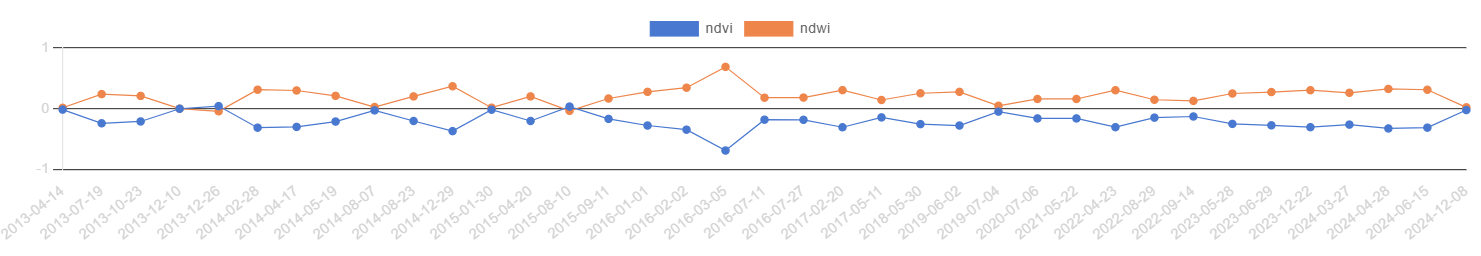
\includegraphics[width=0.97\linewidth]{FIGURAS/graphvisualiser-1747928457345}
	\label{fig:INDICES3}{ Fonte:   Elaborado pelos Autores (2025)}
\end{figure}



% ------
%!TEX root = ..//preambulo.tex
 
\section{Discussão }

 \hspace*{1.25 cm} Na proposta de avaliação dos impactos do lançamento de rejeitos de mineração próximo a foz do rio Doce. Se o local escolhido do estudo, através da técnicas de sensoriamento remoto, nos possibilita inferir as alterações do meio físico: antes, durante e depois do acidente.\\
 %
 \hspace*{1.25 cm} Na primeira hipótese \textbf{\textcolor{blue}{$ H_{\ref{h1}}$}}, avaliou-se se o sensor utilizado consegue discriminar os efeitos do evento. Conforme apresentado nos parágrafos 1 a 4 da seção 4 e nas Figuras \ref{fig:rplot0ndwi2023} a \ref{fig:difer202332026},o índice NDWI revelou alterações perceptíveis na data próxima ao ocorrido, conforme ilustrado na Figura \ref{fig:inda2023}. \\
 %
 \hspace*{1.25 cm} Em segunda hipótese \textbf{\textcolor{blue}{$ H_{\ref{h2}}$}},, buscou-se uma explicação baseada em critérios matemáticos, com menor subjetividade na interpretação. Para tanto, utilizou-se a geoestatística como abordagem principal. \\
 %
 \hspace*{1.25 cm} Inicialmente, a amostragem aleatória de classes de uso do solo foi testada, mas os resultados, avaliados por meio de normalidade, erro amostral, variância, coeficiente de determinação e métrica RMSE, mostraram-se ineficientes, explicando apenas 41\% da variabilidade do modelo espacial.\\
 %
 \hspace*{1.25 cm} Por outro lado, a amostragem em grade ("grid") conseguiu explicar aproximadamente 95\% do modelo. Por isso, essa abordagem foi selecionada para a construção do semivariograma e sua representação espacial, incluindo os desvios-padrão.\\
  %
 \hspace*{1.25 cm} A amplitude geográfica e a maior variabilidade dos resíduos indicaram os locais onde o modelo de superfície tridimensional apresentou menor capacidade explicativa, sendo esses os pontos de maior atenção, com z-scores mais altos \ref{fig:Rplothddg} e desvios mais expressivos, representados por regiões mais escuras no mapa da Figura \ref{fig:rplotkriga}.\\
 %
 \hspace*{1.25 cm} Portanto, a hipótesee \textbf{\textcolor{blue}{$ H_{\ref{h2}}$}} foi confirmada, indicando que o sensor foi sensível ao fenômeno e identificando áreas geográficas que demandam maior esforço de explicação.\\
 %
 \hspace*{1.25 cm} Por fim, a terceira hipótese \textbf{\textcolor{blue}{$ H_{\ref{h3}}$}}.foi considerada a mais direta pelos autores. A extração dos valores de reflectância e seus índices, diretamente sobre os alvos/focos em locais com maior variabilidade temporal, foi ocasionada pelo fenômeno e detectada pelo sensor. Em termos simples, o que foge à normalidade pode ser considerado anômalo.  \\
 %
\hspace*{1.25 cm} As coordenadas geográficas com menores valores de reflectância, em áreas sujeitas a alagamento, apresentaram as maiores distorções de reflectância ao longo do período analisado, conforme demonstrado nas Figuras \ref{fig:INDICES} a \ref{fig:INDICES3}, Após o evento, os valores de reflectância desses alvos retornaram à normalidade.
 
% ------
%!TEX root = ..//preambulo.tex
\section{Conclusão}

\hspace*{1.25 cm}  As Figuras \ref{fig:indao} ilustram a situação local durante a inundação ocorrida em 2013. Já as Figuras \ref{fig:indao2} e \ref{fig:indao3} mostram a chegada de rejeitos à foz do rio Doce. Ambos os fenômenos foram detectados por sensores orbitais e pela população residente.\\
%
\hspace*{1.25 cm} No presente estudo, a dinâmica territorial e espacial afetada pelo despejo de rejeitos de mineração foi analisada, consolidando a hipótese por meio de métodos matemáticos, especificamente a geoestatística, e de um painel temporal que descreve as alterações físicas do fenômeno..\\
% 
\hspace*{1.25 cm} Verificou-se que a amostragem por grade foi a mais apropriada para este estudo. Não ficou claro se a ausência de explicação sobre o modelo de amostragem aleatória decorreu de limitações metodológicas ou da falta de aprofundamento conceitual dessa técnica, uma vez que os procedimentos e algoritmos utilizados foram os mesmos.\\
%
\hspace*{1.25 cm}A função esférica ajustou-se melhor aos dados, e tanto o processo automático, e utilizando krigagem, quanto o processo manual obtiveram parâmetros semelhantes, permitindo descrever os locais geográficos para estudos mais aprofundados. \\
%
\hspace*{1.25 cm} A  Figura \ref{fig:Rplothdg} por meio da modularização para descrição e sumarização estatística da reflectância temporal, foi capaz de destacar pontos discrepantes relacionados ao fenômeno estudado. Esses pontos ou dados anômalos não foram excluídos na Figura \ref{fig:variinical}.\\
%
\hspace*{1.25 cm} Conforme recomendado pela própria metodologia geoestatística, estudos mais aprofundados devem ser direcionados aos locais onde o modelo apresentou dificuldades para explicar os fenômenos observados.

% ------
\addcontentsline{toc}{section}{Referências}
% ----------------------------------------------------------
% ELEMENTOS PÓS-TEXTUAIS
% ----------------------------------------------------------
%\postextual
%\newpage
% ----------------------------------------------------------
% Referências bibliográficas
% ----------------------------------------------------------
\bibliography{Referencias//abntex2-doc}
% ------


% ------
\PrintChanges
\PrintIndex
% ------

% ------
\StopEventually{\PrintIndex}
% ------

\StopEventually{\PrintIndex}
\end{document}

